\documentclass{cshonours}

\usepackage{url}
\usepackage{minted}
\usepackage{hyperref}
\usepackage{enumitem}
\usepackage{graphicx}
\usepackage{pdflscape}
\usepackage[style=alphabetic, sorting=nyt]{biblatex}
\addbibresource{bibliography.bib}

\title{6CCS3PRJ \\\vspace{0.5cm}
  A Pragmatic Infrastructure Modelling and Verification Framework}
\author{Joe Stanton\\\vspace{0.5cm}
  Student ID: 1020836
}

\begin{document}

\maketitle

\chapter*{Abstract}

%Trends:

%* Cloud Computing and Virtualization, LXC Containerization
%* Dynamic, Elastic, Auto-Scaling
%* Configuration Management
%* Immutable Infrastructure
%* Full Stack Monitoring
%* High Level Visualisation of Application Architecture

Application architectures are more complex and dynamic than ever. The growth in cloud computing makes it cheaper and more accessible to build and maintain services at scale, yet the tools to manage the complexity of these services, and their inevitable change over time, are often inadequate.

 Infrastructure complexity is steadily increasing, and is a leading cause of downtime and unreliability. According to a recent Gartner survey, 73\% of IT executives say their infrastructure complexity is either `high' or `out of control'.

In this report, we discuss and implement an infrastructure modelling and monitoring tool that can be used to help manage some of the inherent complexity in modern infrastructure. We will attempt to design an infrastructure modelling language, and use the subsequently produced models to effectively visualise and validate the correctness of real-world systems.

\chapter*{Originality Avowal}
I verify that I am the sole author of this report, except where explicitly stated to the contrary.

I grant the right to King’s College London to make paper and electronic copies of the submitted work for purposes of marking, plagiarism detection and archival, and to upload a copy of the work to Turnitin or another trusted plagiarism detection service. I confirm this report does not exceed 25,000 words.

\textbf{Signed:} Joe Stanton

\textbf{Date:} \today

\chapter*{Acknowledgements}

I would like to express my gratitude to Dr.\ Steffen Zschaler, for agreeing to supervise this project when it was a rather abstract idea. His subsequent useful advice throughout the year has also been invaluable.

\tableofcontents

\chapter{Introduction}

\section{Thesis}
\textit{It is practical and useful to develop an infrastructure modelling and monitoring tool to help address the inherent complexity in modern IT infrastructure.}
\section{Motivation}

After taking part in the delivery of software in the highly regulated insurance industry, I noted some problems with the reliability of the software delivered. These reliability issues were generally unrelated to the application itself, but predominantly caused by the growth in complexity of the underlying application infrastructure, which was provided and managed within the company's own datacenter as a result of regulatory constraints. As the application grew in complexity over time, the number of dependent services and components needed to keep it running became unmanageable by the company's own IT staff.

I discovered a real disparity between the knowledge application developers had of the specific requirements of their application (hardware specifications, dependencies on other services, likely points of failure) and the lack of awareness of this within the operations team. This phenomenon has been noted in other areas of the industry~\cite{DevOps} and has recently given rise to the term `DevOps' - an attempt to improve communication between the teams or build tools that help to do so.

Better collaboration and knowledge transfer between these teams often provides the following benefits:

\begin{description}
  \item [Proactive maintenance of the system and its dependencies]\hfill \\
    The effect of changes is well understood by all members of the team and problems can be foreseen ahead of time. The infrastructure can be modernised progressively.
  \item [Identification of weaknesses in the system architecture]\hfill \\
    e.g.\ single points of failure, overworked or repeatedly unreliable components can be identified, and discussion between the teams can lead to effective solutions.

  \item [Reduced risk of change]\hfill \\
    Delivery of features and bug-fixes to deployed software can happen regularly and reliably through Continuous Delivery.

  \item [Quick and effective root cause analysis]\hfill \\
    When issues do occur, they can be diagnosed and fixed quickly, and then prevented in the future.
\end{description}

\section{Solution Objectives}
%Embracing change is a key tenet of the cloud computing architecture.

The objective is to design and implement a tool that helps with the modelling of complex infrastructure within real-world systems. The application will provide application developers or operations staff the ability to model systems as a graph of interconnected nodes, which may have dependencies and fine grained tests used to verify their current state.

The tool will then execute this model as a means of system monitoring. It will verify the correctness of the live system continuously and warn of any divergence. It will also allow the attachment of meta-data and metrics to nodes. This model, meta-data and metrics will then serve as a useful diagnostic tool if the state of the system changes, e.g.\ a loss of connectivity between two nodes. This fine-grained and clear mechanism of communicating failure should reduce investigation and response times when issues arise, and provide the insight which prevents them from recurring.

This model can serve as `living documentation' that is used by Ops teams and Developers to help manage and transfer knowledge, documenting their implicit knowledge. It should help to predict the impact of changes. It should improve collaboration between the teams and provide deeper insight into issues with the performance or reliability of the system.

Languages and tools for the modelling of software architecture and infrastructure do exist, however they lack the simplicity and pragmatism in their implementation to see widespread adoption in industry~\cite{IndustryMDSE}. I propose a simple, pragmatic tool that may come with some modelling limitations, but will be quick and easy to set up and begin reaping the benefits.

Given its role as the centralised location of knowledge for the system, this tool could become a platform to solve other distributed systems issues, such as service discovery etc.\ but these problems are not part of the initial scope.

\section{Software Platform and Target OS}

The system will be developed in multiple parts and distributed across hosts, where an appropriate choice of programming language will be used to suit the task. The application will generally consist of a web based modelling tool, which also provides feedback on the current state of the system, and a set of background processes that perform the verification and feed changes back to the web interface.

All user interaction will be web based, due to the ease in distributing and updating the system and the lack of an installation step. Latest browsers with HTML5 and CSS3 support will be targeted as these are common amongst IT professionals. More details on the chosen system architecture are presented in \autoref{section:architecture}.

\chapter{Background Research \& Literature Review}

In this chapter, we discuss the increase in infrastructure and software complexity, and how the industry has adapted to deal with it. We also review some literature from related research fields and evaluate the effectiveness of the proposed solutions.

\section{Managing Software Complexity}

The problem of increasing software complexity is a well publicised and researched phenomenon. Software that is complex takes longer to develop, and is harder to maintain. As it affects the value proposition to the user so directly, it is often the dominant factor in determining the feasibility of implementing a given system.

The rise in software complexity together with ever changing business demands during its development has given rise to a number of popular methodologies or techniques in research and industry, such as Model Driven Development~\cite{ModelDrivenDevelopment}, Extreme Programming~\cite{BeckXP} and the Agile movement~\cite{AgileManifesto}.

\subsection{Modelling and Model Driven Software Engineering (MDSE)}

Modelling of complex software has been used for a number of years as a tool of communication between developers, project managers and stakeholders. A number of tools can be used to produce clear diagrams of a system, but models provide a level of semantic meaning that allows them to be practically used to derive or verify an implementation. The Unified Modelling Language is considered the de-facto set of graphic notation techniques to create visual models of object-oriented software-intensive systems~\cite{UMLDefinition}.

\paragraph{Diagrams vs.\ Models}
A drawing tool can only be considered a modelling tool only if the tool `understands' the drawings~\cite[p.~11]{ModelDrivenDevelopment}. This has a number of benefits:

A modelling tool guarantees a minimum level of semantic meaning and model quality, because they grant alignment to some sort of meta-model~\cite[p.~12]{ModelDrivenDevelopment}.
The model can often be used to derive an implementation or perform checks/validation to ensure that a given implementation satisfies the model.


\paragraph{Modelling Techniques}
Models can be built textually as well as graphically. Textual models are commonly expressed using Domain Specific Languages (DSL’s). A DSL is defined as ``a computer programming language of limited expressiveness focused on a particular domain"~\cite{FowlerDSL}. Textual models can still sometimes be used with graphical tooling to provide a visualisation of the expressed model.

\paragraph{Adoption of Modelling and MDSE}

Studies into increased quality, maintainability and developer productivity when using MDSE techniques are found commonly in academia but are difficult to find in industry. In a study into Industrial Adoption of Model Driven Development, it was stated that ``interviewees emphasised tool immaturity, complexity and lack of usability as major barriers to adoption"~\cite{IndustryMDSE}.

\subsection{Unit and Integration Testing}

A popular method of managing software complexity is via the introduction of unit testing. The primary goal of testing is clearly to improve the quality of a delivered piece of software, but unit testing achieves this goal by forcing the decomposition and validation of different parts of the system in isolation. Systems designed with unit testability in mind are commonly more modular and less coupled to the overall system, as this generally makes tests much easier to write.

Edsger W. Dijkstra once stated that ``Simplicity is prerequisite for reliability", simplicity can be achieved by decomposing difficult problems into smaller, more manageable chunks, and unit testing encourages this practice.

Test Driven Development (TDD) has surged in popularity within industry as a result of the XP and Agile movements. The cited benefits are: improved software quality and increased responsiveness to changing customer requirements~\cite{BeckTDD}. TDD further encourages the decomposition of software into smaller, independently verifiable modules, but goes further than this by stating that these tests should be written before the implementation.

There are many types of testing, but they can generally be grouped into two main categories:

\begin{description}
  \item[Unit Testing] The main role of unit testing is as a design tool, developers can write unit tests to specify the intended behaviour of a component and then implement it to match. They provide fast and specific feedback on the correctness of implementation.
  \item[Integration Testing] verification that each separate component of the system functions correctly when it has been integrated with other components. This could range from testing the composition of two small components or an entire order processing pipeline. They are used to improve confidence in overall system correctness, and they are often use to guard against regressions in functionality over time.
\end{description}

We can see many applications of unit/integration testing in the management of infrastructure complexity, as well as software complexity. This observation heavily influences the rest of this report.

\section{Managing Infrastructure Complexity}

There is clearly a large amount of research and analysis into managing software complexity. In this section, we will review the techniques used to manage the infrastructure side of this complexity.

\subsection{General Modelling Tools}

A number of modelling standards are extremely flexible and allow the expression of arbitrary systems. One example of this is the Common Information Model (CIM) standard~\cite{CIM}. There are many IDE’s and tools that have the ability to construct CIM compliant models, such as the Eclipse Modelling Framework~\cite{EMF}.

It is relatively difficult to find practical examples of infrastructure modelling in CIM, making it difficult to get started with unless the user already has experience with MDSE techniques.

Such generic modelling tools are useful for communicating ideas or states of a system, but it could be argued that they lack pragmatic value. It is often not possible to execute the produced models in order to derive an implementation, as a set of transformations from any arbitrary model would prove too complex to implement. The inability to execute these models limits their value significantly.

\subsection{Infrastructure Modelling Tools \& Configuration Management}

Modern configuration management tools can be considered a type of infrastructure modelling tool. Most of these tools such as Puppet~\cite{Puppet}, or Chef\cite{Chef} use a Domain Specific Language to declaratively define hosts, their respective software stack, and install and manage their respective services.

Configuration management tools are especially interesting due to their mass adoption in recent years within the Agile software development community, as well as at enterprises such as Facebook and Amazon~\cite{Chef}.

The real value of these DSL's is that they are directly executable. 
They can be executed to drive infrastructure changes and ensure convergence with the model. Listing~\ref{fig:PuppetDSLSnippet}. provides an example snippet of a Puppet recipe, declaratively specifying details of the SSH (secure shell) service that will be made available on a specific host.

As part of the runtime execution, each service's conformance to this set of properties is verified and if there is any divergence, the tool will orchestrate a set of imperative actions, for example installing the service or altering its configuration file and then restarting it.

\begin{listing}[H]
\begin{minted}[fontfamily=fi4]{ruby}
class sshd {
    package { 'openssh-server':
        ensure => latest
    }
    service { 'ssh':
        subscribe => File[sshdconfig],
        require   => Package['openssh-server'],
    }
    file { 'sshdconfig': 
        name    => '/etc/ssh/sshd_config',
        owner   => root,
        group   => root,
        mode    => 644,
        source  => 'puppet:///sshd/sshd_config',
        require => Package['openssh-server'],
    }
}
\end{minted}
\caption{A puppet recipe snippet, declaratively configuring the SSH service on a host. The execution of this description is idempotent, so can be repeated safely to ensure convergence.}
\label{fig:PuppetDSLSnippet}
\end{listing}

\clearpage
\subsection{Existing Monitoring Tools}

I have extensively researched existing monitoring tools ranging from very simple ping checks to complete enterprise solutions and evaluated their effectiveness. In the interest of brevity, I have included a small sample of popular monitoring tools I have evaluated that give an indication of the cross-section of the market:

\subsubsection{Nagios}

Nagios\footnote{Nagios - http://www.nagios.org/} is an open source infrastructure and application monitoring framework. Often considered the `industry standard', it provides a vast array of features, from execution of fine-grained protocol specific tests to complex capacity planning forecasts. It is also very extensible, which is perhaps the largest reason for its success within the industry.

Nagios is in active use by over 250,000 organisations worldwide, including Amazon, AT\&T and JP Morgan Chase~\cite{NagiosUsage}. It supports a number of common monitoring architectures, including both agent based and agent-less (based on the Simple Network Management Protocol) that means it can run efficiently up to a very large number of hosts~\cite{NagiosArchitectures}.

Anecdotal feedback about Nagios typically suggests that it is a mature and flexible solution for basic monitoring of large numbers of hosts, but severely lacks some higher level concepts such as integration tests of system components. It is also considered extremely time consuming and counter-intuitive to set up and manage, which perhaps explains its lack of adoption within smaller businesses/startups.

\subsubsection{StatsD, CollectD, Graphite}

This collection of tools all work together in providing near real-time metrics tracking and graphing, they are used heavily at vastly successful startups such as 37signals~\cite{37SignalsGraphite} and Etsy~\cite{EtsyGraphite}. Metrics can be collected from the infrastructure and application layers.

\label{StatsD}
Application level metrics can be collected using StatsD\footnote{StatsD - http://codeascraft.com/2011/02/15/measure-anything-measure-everything/}. Applications can send metrics to a local StatsD instance via UDP, which adds very little performance overhead. This means that it is possible to heavily instrument the critical paths of an application except in extremely performance sensitive scenarios. Both of these tools aggregate this data and flush it to a backend Graphite\footnote{Graphite - https://graphite.readthedocs.org/en/latest/overview.html} instance at configurable intervals. Graphite provides extremely flexible data visualisation techniques, but requires some up front investment in time to produce meaningful results.

This collection of tools provides an extremely flexible and performant source of aggregate data that can be used to diagnose reliability and performance problems effectively. Its disadvantages however include a lack of any alerting mechanism, a number of independent components that are both non-trivial to deploy and difficult to monitor themselves, and a difficulty in actually interpreting aggregate data to draw conclusions without deep insight into both the application and the infrastructure it’s relying on.

\subsubsection{New Relic - APM}

New Relic\footnote{New Relic - http://newrelic.com/about} is a popular subscription-based, hosted Application Performance Monitoring (APM) service. It provides integration with popular languages, frameworks and platforms such as the Java Virtual Machine (JVM), Ruby/Ruby on Rails and Python with the Django web framework.

New Relic is extremely easy to integrate with existing web applications as it provides environment specific tooling such as Ruby gems or Python packages. It reports on fine-grained application metrics such as slow SQL queries, poor response times and browser based monitoring metrics with a snippet of JavaScript.

Whilst New Relic is simple to set up and provides a fairly deep insight into application performance, it is a relatively expensive service beyond a trivial number of hosts and severely lacks the extensibility of the open source solutions when it comes to monitoring other non-supported parts of the stack.

\subsubsection{Summary}

A vast array of monitoring tools already exist, many of which are mature solutions. However, they generally require a large investment of time and do not help with visualising or managing infrastructure complexity. They often also require deep insight into the application/service being monitored, which is not always the case when developers and operations teams are separate.

An ideal solution would be an open source tool, incorporating the ease of setup of a service like New Relic, with the flexibility and alerting of Nagios and Graphite. It would also provide a holistic view of the system and its dependencies so it is easy to visually identify problems and their effects without deep insight into the application architecture.


\chapter{Requirements Specification}

A set of functional and non-functional requirements will be established from user stories based on my own personal experiences developing software in industry, and conversations with the following typical target users of the system:

\begin{itemize}
  \item A Technical Architect at Red Badger Consulting
  \item A System Administrator at HCL
\end{itemize}

\section{User Stories}
\begin{enumerate}
  \item As a developer, I would like a simple and expressive way to document my application's infrastructure requirements, so I can effectively communicate them to other developers and system administrators.
  \item As a developer, I have the ability to execute my documented infrastructure specifications to automatically validate the correctness of the system under test.
  \item As a developer, I can express arbitrary properties that the system under test must satisfy, while making use of open source libraries. So I can quickly produce accurate and practically useful specifications.
  \item As a system administrator, I can see a clear overview of the system, detailing its architecture and dependencies, so I can understand and effectively support it.
  \item As a developer / system administrator, I would like to verify the state of the system under test continuously, so I can quickly identify and resolve problems when they occur and make the system more amenable to change.
  \item As a developer / system administrator, I would like to capture changes within the system as they occur, such as code deployments or re-configuration, so I can relate these events to issues that may occur, making root cause analysis easier.
  \item As a developer / system administrator, I would like to be notified of changes in the state of the system via email and SMS, so I can respond to incidents quickly.
  \item As a system administrator, I would like to easily create specifications for applications I have already deployed.
  \item As a developer / system administrator, I would like to measure the reliability of a service and its components over time.
\end{enumerate}

\section{Functional Requirements}
\begin{enumerate}
  \item Testing Framework
    \begin{enumerate}
      \item The developer should be able to install the tool on their development workstation and servers.
      \item The developer should be able to use to the tool to describe a system accurately and concisely.
      \item The developer should be able to execute this description to validate the correctness of a system, verifying any arbitrary property as required.
      \item The tool should provide an auto-detection process to detect existing services and assist in describing them.
      \item The tool should provide built in checks so the developer does not have to write them all from scratch.
      \item The developer should be able to use external libraries to add additional functionality to health checks.
      \item The developer should be able to deploy this tool on a production server, and monitor the system continuously.
      \item The tool should report results back to a central location where they can be viewed.
      \item The tool should work in an environment where inbound connections to the system under test are prohibited by a firewall.
    \end{enumerate}
  \item Data Collection and Monitoring
    \begin{enumerate}
      \item The tool should effectively visualise the state of a system under test, including services, components and hosts.
      \item The tool should provide a way to view results of the health checks.
      \item The tool should provide a way to track and visualise changes happening within the system.
      \item The tool should calculate the degree of reliability of each host, service and component.
      \item The tool should send Email notifications to users when incidents occur.
      \item The tool should send SMS notifications to users when incidents occur.
      \item The data collection and monitoring should be deployable on a private network.
    \end{enumerate}
\end{enumerate}

\section{Non-Functional Requirements}
\begin{enumerate}
  \item Reliability - The system and all of its components should provide a reliable platform for monitoring live systems.
  \item Usability - It should be easy to start using the system and understand how it fits within the users existing organisation. Understanding of the implementation details should not be necessary for basic use cases.
  \item Performance
    \begin{enumerate}
      \item The system should efficiently validate system correctness.
      \item Alerts or warnings should be delivered in a reliable and timely fashion.
      \item Validation of the system should scale above a trivial number of hosts. (Over 20)
      \item The impact of validating correctness on the system under test should be minimal.\ i.e. no significant degradation in performance of the monitored applications or resource exhaustion of the hosts under test.
    \end{enumerate}
  \item Security - The system is intended for use in production environments, therefore it should not unnecessarily expose the target system to threats such as the following:
    \begin{enumerate}
      \item Open network ports
      \item Insecure transmission of sensitive data
      \item Remote code execution
    \end{enumerate}
  \item Maintainability - The system should be maintainable so that new features are easier to implement and the implementation is easier to understand for any open source contributors.
    \begin{enumerate}
      \item Separation of Concerns - The system should be decomposed into a number of separate components which can be built and tested in isolation. They may use different languages and frameworks as appropriate for the specific task.
      \item Architectural Patterns - The system should make good use of appropriate design patterns and architectural techniques provided in the implementation language, such as encapsulation and composition in an object orientated language.
      \item Unit Testing - Wherever possible, the code should be tested by a suite of unit tests that achieve a high coverage of the total codebase.
    \end{enumerate}
  \item Interoperability - The system should integrate with existing systems in order to provide maximum flexibility/utility to the users. It should therefore:
    \begin{enumerate}
      \item Provide a simple interface such as a HTTP API to read and write data
      \item Expose data in a standard format such as XML or JSON
    \end{enumerate}
\end{enumerate}

\section{Additional Aims}

I will open source the project on GitHub, using a flexible and open license, as it could appeal to anyone with a general interest in infrastructure modelling and verification. Similar to a unit testing framework, the project would be pitched as a distributed modelling and testing framework for servers and other infrastructure. Open sourcing the project could have a number of benefits, such as:

\begin{itemize}
  \item Encouraging feedback and iterative improvement.
  \item The opportunity to build a community of contributors and plugins.
  \item Increased incentive to integrate with other open source DevOps tools such as Chef or Puppet.
  \item Better chances of adoption, as the tool would be free to use, modify and re-distribute.
\end{itemize}

If the project is open sourced, it could still be made available commercially in a hosted and supported form at a later date.

\section{Limitations}

Due to the significant differences between Windows and UNIX based servers, including compatibility of tools, remote command execution strategies and scriptability, I have decided to target only UNIX based (specifically Linux) servers initially. This decision is based upon the dominance of UNIX within the server market, at 66.8\% in a 2013 study~\cite{UnixMarketShare}.

The platform limitation will apply to the first version of the tool, but it will be possible to implement a layer of Windows compatibility for verification using a scripting interface such as PowerShell, given extra development time. This enhancement is potentially a good candidate for an open source contribution.

\chapter{Design and Implementation}

The following chapter details the design and implementation process. It specifically focuses on the the critical technical decisions made, and how they relate back to the requirements and design objectives set out initially.

\section{Design Objectives}

\paragraph{Speed/Ease of Setup} Comments from developers often mention that most monitoring and modelling tools were too time consuming to set up. Clients did not see demonstrable value in investing time upfront in this process before services were launched and issues actually occurred.

A tool that provides a simple installation process, follows ‘convention over configuration’ and provides a degree of auto-detection of installed services would be extremely valuable and increase chances of adoption significantly.

\paragraph{Simplicity and Pragmatism} Often the need for extensive application and infrastructure monitoring is not fully recognised until after the application has been deployed into a production environment. Introducing monitoring at an earlier stage, e.g.. in a staging environment, can highlight issues of reliability and performance before they are experienced in production. Monitoring key domain specific metrics can also aid in reasoning about the runtime behaviour of the system. With these benefits in mind, the tool should be simple enough to introduce early in the development process with minimal effort on the part of the developer, it should provide pragmatic value from the start, and offer the flexibility to continue to deliver value as the system grows in complexity.

\paragraph{Embracing Change}

Maintaining agility while providing a suitable quality of service is challenging. Continuous Integration (CI) and Delivery (CD) are fundamental principles of the Extreme Programming\cite{BeckXP} (XP) movement and discuss solutions to this problem at great length, the most cited benefit is the reduction of risk. Small amounts of change applied frequently are easier to reason about and test, and of course provide the end user with value quicker. In conjunction with version control systems, CI/CD can be used to effectively identify the root cause of problems soon after they occur. The application of CI/CD is widespread within the industry, and a whole suite of tools such as CI servers, automated code deployment tools and configuration management utilities all aid to facilitate the practice.

The monitoring tool should fit within an agile workflow, where system architectures change frequently. It could even be used to verify that system reconfiguration was successful, as a form of test driven infrastructure change. The tool should provide the means to track changes such as code deployments and re-configuration and provide an interface to visualise this, similar to viewing changes in code under source control.

\paragraph{Dynamic Infrastructure}

The nature of modern infrastructure is no longer static. Cloud computing and virtualization provide the means to scale different parts of the system independently and automatically. For example, Amazon AWS provides `auto-scaling groups' that create new instances of an application according to pre-defined load thresholds. Capturing and visualising these changes is something that existing monitoring tools struggle with, as they are aimed at more traditional, static infrastructure. The tool should provide the means for tracking these changes.

\paragraph{Flexibility}

It is imperative that monitoring tools do not just focus on common areas that are easy to measure or verify. The monitoring needs of an application could be highly domain specific, and overly simplistic verification can cause misleading results. The tool must provide the means to encode and verify arbitrary properties of the system at varying granularity. One reason that distributed systems are much more difficult to debug is the non-determinism introduced by unreliable networks, layers of caching and load balancing. It should be possible to bypass many of these sources of non-determinism so that real issues can be highlighted. It should do this in the same way as a good unit testing framework does, with the full capability of a programming language, leveraging a vast array of existing open source libraries.

\paragraph{Streaming Metrics} The vast majority of monitoring tools are based upon a polling mechanism. Configured checks are performed from a centralised server at pre-defined intervals. Reversing this mechanism so that servers stream their own metrics back to the monitoring server addresses a number of issues with polling such as the following:

\begin{itemize}
  \item Firewall Reconfiguration - Typically firewalls do not allow inbound connections except where explicitly defined by a rule. This means that monitoring tools will not work until rules are explicitly added for them. Outbound connections usually do not suffer from this constraint, and therefore do not require reconfiguration of existing infrastructure.
  \item Poor Scalability - Performing checks from a single server does not scale to a large number of hosts, typically the solution for this is to increase polling intervals to reduce load. Streaming places the overhead on each server being monitored, where it can easily be tolerated. The management server should easily be able to process a stream of results from a very large number of hosts, and where this becomes less feasible, this could be load balanced.
  \item Polling Latency - If checks are scheduled infrequently, there is an artificial time delay in receiving notifications. Not only does this mean that issues are not identified as quickly, but the slow feedback can be confusing when attempts are made to fix the underlying problem.
\end{itemize}

\paragraph{Hosted vs. On-Premise Solutions} The system should be built and packaged so that it could run as a hosted service (typically more suitable for startups, and easier to experiment with) and as an on-premise solution where there are concerns over data security or scalability. This can be achieved by using a configuration management tool for setup and deployment, which also has the capability to produce, as build artifacts, pre-built system images such as VMWare packaged appliances or Amazon Machine Images (AMI's).

\paragraph{Security} The installation of any networked monitoring tool increases the attack surface-area on production systems that often host important services and contain sensitive user data. In order to partially mitigate this concern, communication between the each node and the monitoring system will be encrypted, and both the server and client must verify each other’s respective identities to ensure that no Man in the Middle (MiTM) or general spoofing/poisoning attacks can become effective.

Public-Key cryptography can generally provide this functionality, if the agent installation is performed via HTTPS, the identity of the management server can be verified and a public key can be exchanged from this point forwards in all communication. In addition, communication between the nodes after initial setup is uni-directional, for the purposes of reporting metrics, so the monitoring agent does not need to listen on any network interfaces where it could be compromised.

This strategy needs to be carefully evaluated and tested, but should not present a major risk to the implementation. The difficulty will lie in expressing this capability to future users of the system so they can be confident in its security.

\pagebreak
\section{Domain Model and Concepts}

Based on decomposition of the problem, the following concepts are deemed to be relevant:

\begin{itemize}
  \item Service - An application that provides functionality to an end-user or another service over a network. e.g. a website or API.
  \item Component - Part of a service that performs a specific function, e.g.\ an application server or a load balancer.
  \item Host - A physical, virtual or otherwise isolated container responsible for running some or all of the components of a service.
  \item Metric - A measure of a characteristic at a given point in time, e.g.\ CPU load or average request latency. Typically quantitative in nature.
  \item Check - Validation that an arbitrary property holds at a given point in time, e.g.\ A specific service is listening on port 80. Typically qualitative in nature.
  \item Event - A discrete action performed upon the system, e.g.\ a code deployment or service re-configuration. Events can be correlated with metrics.
  \item Incident - A specific type of event that is automatically triggered by the failure of one or more checks, incidents correlate recent events with failed checks and can be related to previous incidents of a similar nature to aid in root-cause analysis.
  \item Context - Additional data that aids in root-cause analysis, e.g.\ log files from a malfunctioning service.
\end{itemize}

\pagebreak
\section{System Architecture}

\label{section:architecture}

The nature of the system is inherently distributed. Service specifications are written by a developer on their personal machines, must be executed on any number of target servers and have results returned to a centralised location. The following decomposition of components is suggested, with further explanation provided below:

\begin{listing}[h]
  \centerline{
    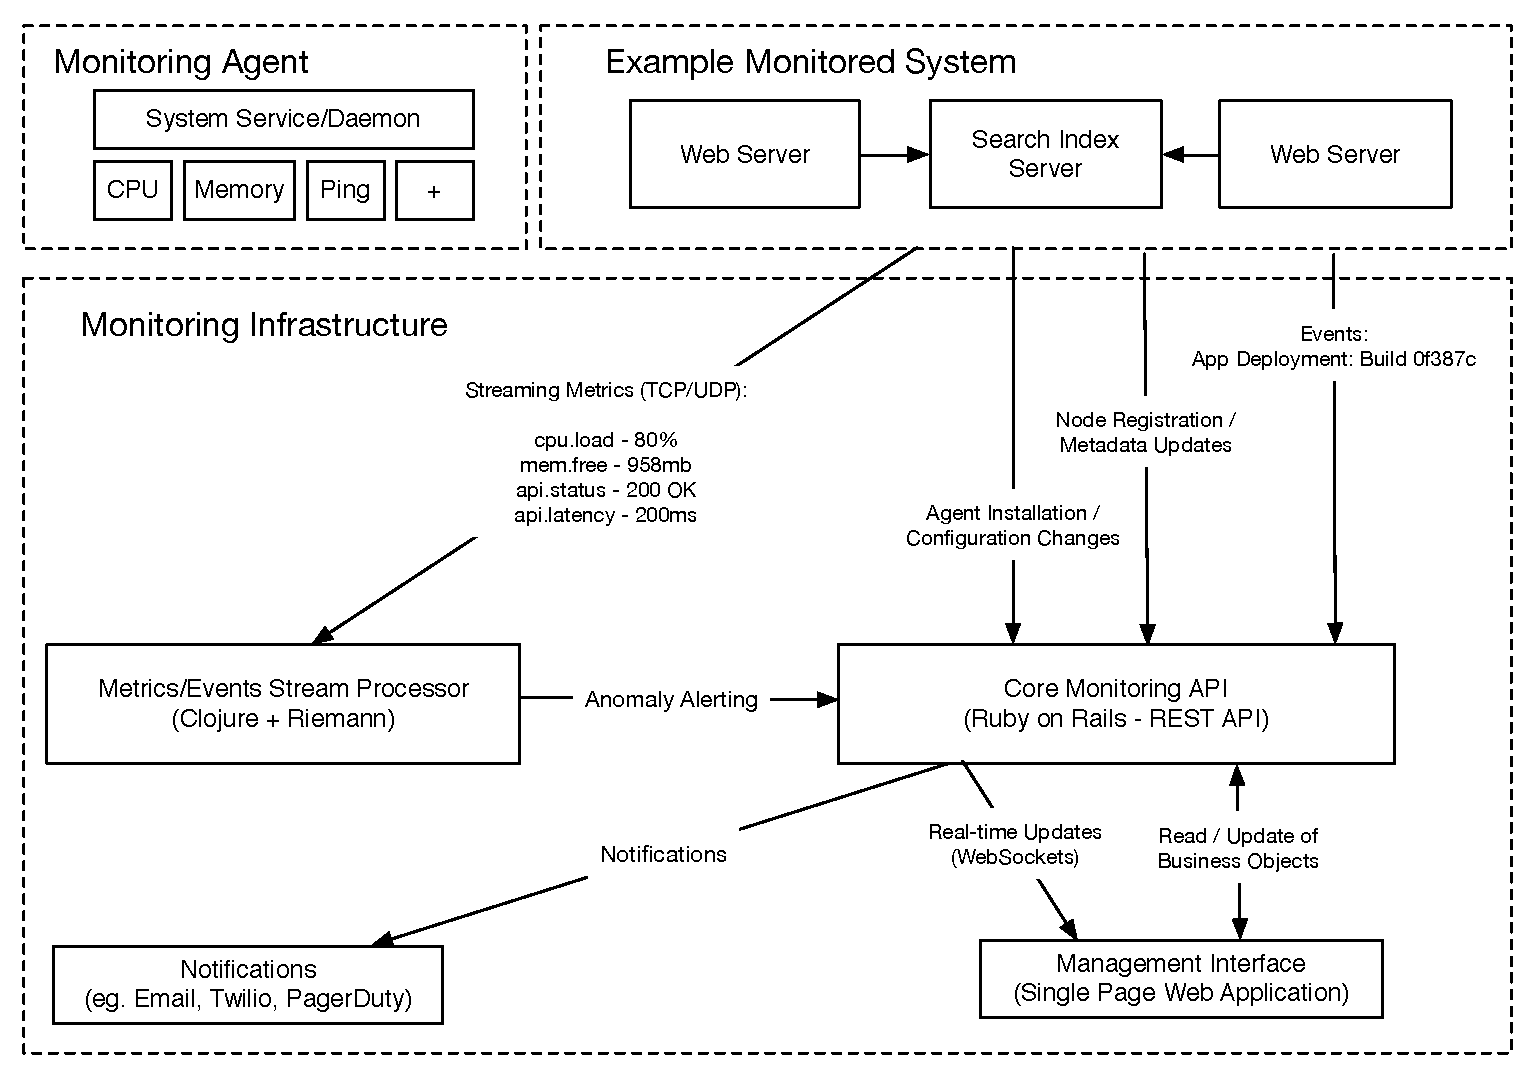
\includegraphics[scale=0.6]{architecture.pdf}
  }
\end{listing}

\subsection{Core Management API}

The API is considered to be the central component of the system, it consists of a database containing all entities such as hosts, services and their respective dependencies. It contains the fundamental business logic for calculating reliability metrics, and triggering events or alerts. It acts as the point of integration for all other components, as well as for external services. It is exposed as a HTTP REST API, which will accept and return data in a standard format such as JSON or XML.

The Management API should support a mechanism of real-time updates, such as a WebSocket or Server Sent Event connection which broadcasts significant changes in the system so they can be displayed by any connected clients.

\subsection{Streaming Metrics/Events Service}

The streaming service manages the collection of check results, metrics or logs via event streams over TCP or UDP\@. Streams reporting errors or anomalous metrics will trigger status changes in the management API, as will streams that stop receiving messages, as this may indicate failure in the monitoring framework itself. The streaming service should be the most scalable component, as it will likely be the limiting factor in the total number of checks/hosts supported by the system.

The API itself could assume this role, but the number of events received could become very high and overwhelm it. When considering that a very large percentage of events will be identical to previous events, it makes sense only for the significant events to be forwarded to the API.

Due to its highly parallel and asynchronous nature, this service will be written in Clojure, as the functional programming style and asynchronous primitives within the language make it an ideal candidate for this type of processing. The Riemann ~\cite{Riemann} event aggregation and stream processing library has been chosen for stream buffering and filtering, the rationale for this choice is expanded upon in the next section.

\subsection{Monitoring Agent}

The server agent is a lightweight component written in Ruby and installed on each server and developer machine. The agent will provide the functionality needed for a developer to create or generate service specifications, expressing arbitrary properties of the system under test that can be automatically verified.

The agent software will be responsible for the execution of checks and the collection of their results. It will forward these results on to the streaming service continuously. The monitoring agent will delegate the execution of checks to any number of bundled plugins, making data collection highly flexible.

\subsection{Web UI}

The web interface is the only user facing component of the system. It is a single page application written in JavaScript, and uses the Facebook React.js library for event handling and data binding, providing structure and testability to the frontend code. It will fetch required data from the management API via AJAX. Where interactive visualisations are used, the D3.js library is used to draw these graphics as Scalable Vector Graphics (SVG).

The Web UI will subscribe to a real-time connection (via WebSockets or Server Sent Events) to listen for changes in the system, this will ensure that any changes in the system are immediately visible to the end user, a feature that many other monitoring systems do not provide.

\pagebreak
\section{Domain-Specific Language}

Providing the flexibility needed to encode arbitrary checks within the monitoring tool is difficult to achieve without a very large amount of static configuration. The full expressive power of a real programming language, leveraging a vast array of open source libraries is perhaps a better way to approach this problem.

Due to its meta-programming features and flexibility in syntax, Ruby is somewhat uniquely amenable to creating domain specific languages within the language itself, so called `internal DSLs'\footnote{Internal/Embedded DSL's - http://www.martinfowler.com/bliki/DomainSpecificLanguage.html}.

The DSL is heavily inspired by a similar DSL of the RSpec unit testing framework ~\cite{RSpec}, RSpec is extremely popular within the Ruby community as it leads to highly-readable test cases. The similarities should provide a common medium for communicating the monitoring tool to those who have used RSpec or similar in the past.

\subsection{Meta-Programming}

Ruby features typically leveraged to create internal DSL's are among the following:

\begin{itemize}
  \item{Blocks} - A fairly common feature of most languages today, Ruby supports `blocks' as an implementation of first-class functions. First-class functions can be used as values, and therefore passed around and evaluated at will.

  \item{instance\_eval} - This function executes a given block in the context of the receiving object. This means that lots of typical structural techniques such as defining classes and methods can be hidden as part of the implementation, and relied upon during execution. This results in readability improvements when used correctly. It is quite similar to the ``fluent interfaces" style~\cite{FluentInterfaces}. An example of this is included below:

  \begin{minted}[fontfamily=fi4]{ruby}
  # Internal DSL implementation
  class Service
    def description(value)
      @description = value
    end
  end

  def service(&block)
    Service.new.instance_eval(&block)
  end

  # DSL interface
  service do
    description "An example service"
  end
  \end{minted}
  \label{fig:MetaProgrammingSnippet}

  \item{method\_missing} - As a dynamically typed language, function calls in Ruby are dynamically dispatched depending on the type of an object. The mechanism for dynamic dispatch also includes a fallback feature used when there are no matching methods with the given name. This means that DSL's can be expressed that pattern match on method names or provide transparent proxies to other objects. Both of these features can be used extensively to create concise, readable DSL's.
\end{itemize}

\subsection{Features and Implementation}

The DSL supports the construction of \textbf{services} and \textbf{components}, they can also be nested, making the hierarchy easy to understand:

\begin{minted}[fontfamily=fi4]{ruby}
  service "Example Service" do
    description "A website"

    component "Nginx" do
      description "The web server"
    end
  end
\end{minted}
\label{fig:MetaProgrammingSnippet}

The most important feature of the DSL is the ability to encode checks as Ruby blocks. A block contains one or more assertions that throw exceptions with descriptive error messages if they fail. Below is a simple example of this:

\begin{minted}[fontfamily=fi4]{ruby}
  service "Example Service" do
    health(interval: 30) do
      running "example-service"
      listening 80
      success "http://example.com"
    end
  end
\end{minted}

The health check will be executed every 30 seconds by the monitoring agent. The monitoring agent will catch any exceptions and return a descriptive error message, which may be printed to the console or serialised and sent to the event stream.

Importantly, as the blocks executed are pure Ruby code that can throw exceptions, any arbitrary code that fits these criterion can be used within a block, including standard expressions and the use of external libraries as plugins:

\begin{minted}[fontfamily=fi4]{ruby}
  service "Example Service" do
    health(interval: 30) do
      ssl_expiry_date < DateTime.now or fail "SSL certificate expired"

      require "redis" # External RubyGem
      Redis.new.ping == "PONG" or fail "Redis is not responding"
    end
  end
\end{minted}

With these simple but powerful primitives, an accurate executable model of the system can be constructed and used for validation purposes. When constructing these service specifications, the agent software can execute all checks on demand so that they can be tested before deployment to a large number of hosts.

This code as configuration approach to monitoring provides a very similar experience to writing unit tests. It can be placed under source control within the existing project repository and therefore fit easily with an existing development workflow, this was a core design goal of the project.

\pagebreak
\section{Monitoring Agent}

The monitoring agent is written in Ruby, and is packaged as a RubyGem. As the monitoring agent is responsible for executing the Domain Specific Language outlined in the previous section, it must be written in Ruby itself or package the Ruby runtime. Despite the fact that Ruby is not typically pre-installed on servers, it is very simple to install and requires no configuration. The installation procedure manages the installation of Ruby if necessary.

\subsection{Installation}

Ease of installation was a core principle of this system, getting started is a one line bash command:

\label{bashinstall}
\begin{minted}[fontfamily=fi4]{bash}
  curl -s https://management-server/agent/install | sh
\end{minted}

Importantly, the installation of the management software occurs over HTTPS, this provides assurances of host identity. The management server must present a valid certificate, mitigating concerns against man-in-the-middle (MiTM) attacks. If this was not the case, it would create an attack vector whereby arbitrary code could be executed on the deployed servers at the point of installation.

The installation script performs the following steps:

\begin{enumerate}
  \item{Detection of Operating System} - The tool initially supports Linux and Mac OS X only, it will distinguish between these operating systems or abort the installation if running on a different platform.
  \item{Detection or Installation of Ruby} - If Ruby 2.0 or higher is not installed, the script will use the standard package manager of the distribution to install it.
  \item{Download of Agent Software} - The source code will be obtained directly from GitHub over a secure connection protecting against spoofing attacks, dependencies will be resolved and installed.
  \item{Host Registration} - Optionally, the host can be registered with the management server, the hostname and IP address as well as an optional service name and environment will be passed to the management server. This is appropriate on servers but not development workstations, as these are irrelevant to the system under test.
\end{enumerate}

\subsection{Workflow}

After installation, a service can be specified and monitored in the following way:

\begin{description}
  \item[Creation or Discovery] The tool is used to create a service specification, either manually or using the service discovery feature.
  \item[Local Testing] The specification is checked for validity on the local machine, ensuring that checks are valid and test for the desired properties. Iterative improvements can be made.
  \item[Pushing] The service definition is pushed to the configured management server, where it is used to update the data model and therefore the user interface. The file is interpreted and posted to the API as a series of partial updates. The original file is also sent, so comments and formatting are maintained for future reference.
  \item[Pulling] Where other hosts provide the same service, they can ``pull" the service configuration from the management server, taking a copy of the original file. They will then be notified of subsequent pushes, ensuring the specifications stay in sync. If this is not appropriate, this role can be fulfilled by an application deployment or configuration management process.
  \item[Monitoring] Monitoring is started on the host, from this point onward, checks will be executed as appropriate and reported back to the management server. Unexpectedly terminating this process will lead to incident alerts.
\end{description}

\subsection{Commands and Usage}

The following commands can be executed from the command-line of a development workstation or server where the management agent has been installed. An example command invocation would be structured as follows: `baseline-agent $<$command$>$"

\begin{description}
  \item[Check] - Run configured health checks on demand. This command is typically used on developer workstations as they iteratively build a service specification using the DSL\@. It provides fast feedback similar to running a suite of unit tests and can be used to quickly validate assumptions, before pushing the specification to the management server.
  \item[Discover] - Creates a service specification from detected system services. This feature can be used primarily to reverse-engineer existing infrastructure setups into a service specification. More details about the discovery mechanism are provided in the next subsection.
  \item[Graph] - Render a graph of the current service - This can be primarily used on the developer workstation, it will use the GraphViz library to render a graph of the system and its dependencies in PDF format. This can be used on its own as a form of documentation, but is typically intended to help visualise the service specification and its dependencies to ensure its correctness.
  \item[Push] - Pushes the specified service to a management server - This command will parse the DSL and serialise each object to JSON, it is then sent as a PUT request to the management API\@. Changes to the service specification take effect immediately and update any connected users in near real-time.
  \item[Pull] - Pulls an existing service from the management server - This command will download the original service specification file from a previous `push" command. This can be used to conveniently add new hosts to existing services.
  \item[Setup] - Register this host with the management server - This is used on the servers running the system under test, it will associate a host with a defined service, listing it in the Web UI and accepting events and check data from it.
  \item[Start] - Starts a monitoring daemon process, which runs in the background and executes checks according to their defined intervals. It will report all data back to the management server's event stream endpoint. Any errors occurring during this process will be logged to a file for later analysis.
  \item[Stop] - Stop monitoring the specified service.
  \item[Restart] - Restart monitoring of the specified service.
  \item[Help] - Describes the function of all available commands.
\end{description}

\pagebreak
\subsection{Service Discovery}

Reverse-engineering a system configuration is a non-trivial task. As this is not the primary intention of the tool, a simple approach is used to detect commonly installed services and provide some common default health checks for them. It relies upon standard UNIX commands such as `ps'\footnote{ps - Retrieves the current process table}, `lsof'\footnote{lsof - Lists open 'file descriptors'} and `netstat'\footnote{netstat - Lists network status, including listening processes} to detect running services.

The algorithm reads from a list of component definitions similar to the following:

\begin{minted}[fontfamily=fi4]{yaml}
database:
  Postgres:
    process: postgres
    description: relational database
    ports: 5432
    version: postgres --version | cut -d ' ' -f3
  MySQL:
    process: mysqld
    description: relational database
    ports: 3306
    version: mysql --version
\end{minted}

It then gets the table of currently executing processes, via the UNIX command `ps aux' and parses the output. It then matches this list with the processes in the service definitions list, and verifies the listening port via `lsof -i :$<$port$>$'.

When a process has been detected, the tool will execute the specified `version' command to extract the current version number of the service.

\pagebreak
The discovery process will output a service specification similar to the following:

\begin{minted}[fontfamily=fi4]{ruby}
service "<Service Name>" do
  component "Postgres" do
    description "relational database"
    type :database
    version "9.3.3"

    health do
      running "postgres"
      listening 5432
    end
  end
  component "ElasticSearch" do
    description "open source search and analytics engine"
    type :database
    version "1.0.1"

    health do
      running "elasticsearch"
      listening 9200
    end
  end
end
\end{minted}

This service specification not only lists the running services, but provides a suggested set of health checks for them, as appropriate. This can help new users of the tool become familiar with the syntax and features of the DSL.

\pagebreak
\subsection{Bundled Checks \& Extensibility}
\label{bundledchecks}

The tool bundles a number of built in checks for common use cases, they can be used by calling methods of the same name, such as:

\begin{itemize}
  \item {Running} - Confirms that a process is running. A process can quit unexpectedly for a number of reasons including misconfiguration, resource constraints, and application errors.
  \item {Listening} - Confirms that a process is listening on the specified network port.
  \item {HTTP Success} - Confirms that a HTTP endpoint responds with a successful status code, that is, one that falls within the 200-300 range when redirects are followed.
  \item {CPU Load} - Uses the systems 5 minute load average to determine CPU utilisation, scaled to the number of CPU's. A high figure can suggest that the current CPU specification is insufficient to support the application.
  \item {Process CPU Load} - Returns the current CPU utilisation for a particular process, useful in identifying processes that are behaving incorrectly.
  \item {Memory Usage} - Returns the total amount of free memory, this metric is sometimes less informative due to aggressive caching and memory management behaviour of modern Linux kernels.
  \item {Process Memory Usage} - Returns the total amount of memory used by a particular process, useful in identifying processes that are behaving incorrectly.
  \item {Disk Usage} - Returns the disk usage specifics for a given mount point. Useful for identifying overflowing log files or under specified hardware resources.
\end{itemize}

\pagebreak
\section{Streaming Event Service}

The streaming event service is designed to collect metrics from a large number of monitored hosts and report any significant changes back to the management API\@. A language with strong support for concurrency and high throughput networking would be ideal for this problem. Ruby has relatively poor support for the above features, as it generally lacks support for non-blocking operations, and has a number of flaws with multi-threading, such as the ``Global Interpreter Lock" problem~\cite{RubyGIL}. In contrast, languages such Java and Clojure\footnote{See http://clojure.org for a full description of Clojure} have far better support for this type of application.

Both Java itself and Clojure have a number of similarities, they both use the Java Virtual Machine (JVM) as the host platform and therefore benefit from a mature ecosystem of tooling and open source libraries. The main difference is that Clojure is a functional language, bringing benefits of improved testability, immutability of data, and higher level concurrency features such as Software Transactional Memory, this makes it a natural fit the problem of transforming and filtering event data concurrently. As Clojure is a good fit for this type of problem, there are a couple of popular libraries suiting this task already. One of these libraries is Riemann\footnote{See http://riemann.io/concepts for an introduction to Riemann.}.

Riemann is a simple and scalable event processing framework written in Clojure, benchmarks suggest that it can process over 200,000 events/sec~\cite{Aphyr200k}. Riemann simply provides a powerful set of primitive operations to filter, throttle and detect changes in streams of data. Custom handling of events is provided via a configuration file, itself interpreted as Clojure. As Riemann provides a vast library of event processing functions, it significantly reduces the amount of functionality needing to be implemented. Both Clojure and Riemann were selected as appropriate implementation choices for this service.

\subsection{Event Schema \& Routing}

Events are sent from the monitoring agent installed on each host via a TCP socket. They use the `Protocol Buffers'\footnote{See https://developers.google.com/protocol-buffers/docs/overview for an introduction} binary format developed at Google to efficiently transport the data.

A typical event payload can be arbitrarily defined, but is typically structured as follows:

\label{eventschema}
\begin{minted}[fontfamily=fi4]{yaml}
  host: "example-production-1"
  service: "example-service"
  component: "nginx"
  description: "Error: Process nginx not listening on port 80"
  state: "error"
  metric: 0
  type: "component"
  tags: ['check']
  notify_endpoint: "/example-service/components/nginx"
  ttl: 15
\end{minted}

The streaming event service provides one endpoint to send all types of event data, for example: results from status checks, application performance metrics and log file entries. These types of event can all be processed and routed to a number of locations. This agnosticism makes it easy to adapt the monitoring architecture in future, hosts can be configured to send data to a single endpoint, which in turn can route the events to their appropriate location.

Another important principle of Riemann is the notion of a time-to-live (TTL) sent with each event. After the number of seconds specified in the TTL field, specified by the sender, Riemann will change the event type to `expired'. This means that if the agent software stops sending events due to a loss of connectivity or a software defect, some error handling logic can be executed, such as updating the component's state to `unknown'. Without this feature, the streaming mechanism would not match the polling based mechanism for robustness.

Checks and performance data are checked for state changes or anomalies before being forwarded to Graphite, a time series database for long term storage and queries. The introduction of Graphite integration means that the framework provides a gradual roadmap to scaling up monitoring granularity and metrics collection. More complex metrics such as median and percentile based performance data can be queried from Graphite and used for anomaly detection.

\subsection{Interpreting Check Results}

Check results are interpreted in the following way:

\begin{enumerate}
  \item The main event stream is filtered down to events with the tag `check'.
  \item The `metric' field of the event is forwarded to Graphite, under an appropriate path, e.g. `example-service.nginx.health'. In the case of health checks, the value is simply 0 or 1, signifying failure or success respectively.
  \item If the most recent event has a different `state' field to the previous event of the same type, queue a notify task. This could happen when a check transitions state due to an error, or where another check packet was not received within the expected TTL interval.

    The number of events matching these criteria is very low relative to the total number of events, and therefore most events never reach the management API. This is a deliberate design decision, as the management API is significantly less capable of handling a high frequency of updates.
  \item The notify task sends a HTTP PATCH request to the management API at the endpoint specified in `notify\_endpoint' signifying a partial update with the new component status. If the status is `error', the request will also contain a description of the error that occurred. This error is often specific enough to pinpoint exact problems within failed components, but this depends on the granularity of the checks involved.
\end{enumerate}

\begin{listing}[htbp]
\begin{minted}[fontfamily=fi4]{clojure}
; Forward all events to graphite, and check for state changes
(streams
  (tagged "check"
    forward-graphite
    (by [:host :service :component :type]
            (changed :state notify-async))))

; Adds events to an async queue
(def notify-async (async-queue! :notify {:queue-size 1000} notify))

; Send a PATCH request to the monitoring API updating the status
(defn notify [event]
  (client/patch (notify-url (:notify_endpoint event))
     {
       :body (json/generate-string {
         (:type event) {:status (:state event) }
     })
     :content-type :json
     :accept :json
   }))
\end{minted}
\end{listing}

\pagebreak
\section{Management API}

The Management API is provided as the interface to the core application logic and domain model. It is responsible for storage and retrieval of all entities such as hosts, services and their respective dependencies. These entities are exposed via the REST API to other parts of the application. The API accepts and responds with JSON\footnote{JSON - http://www.json.org/js.html} serialised data. The API is simple and discoverable, encouraging integration with other systems.

\subsection{Ruby on Rails}

Ruby on Rails\footnote{Ruby on Rails - http://rubyonrails.org/} is an extremely popular web framework written in Ruby. It provides a full suite of functionality from database access to view rendering. It has an extremely active community, over 3,400 contributors\cite{RailsContrib} and has been downloaded nearly 34 million times according to RubyGems.org~\cite{RailsPopularity}. It embraces common best practice patterns such as Model-View-Controller (MVC) and the ActiveRecord pattern~\cite{ActiveRecord}. Ruby on Rails was chosen for this project for the above reasons, as well as the excellent support for testing libraries such as RSpec\footnote{RSpec - https://relishapp.com/rspec}.

Sinatra\footnote{Sinatra - http://www.sinatrarb.com/} and Padrino\footnote{Padrino - http://www.padrinorb.com/} are alternative popular web frameworks for Ruby. Both of these frameworks are more minimal than Rails. They are useful for projects that are either especially simple, or projects that deviate from the standard Rails functionality by a large degree. This is not true of the monitoring API, it is a typical web application that can benefit from many of the framework features Rails offers, therefore it was deemed an appropriate choice for this component.

Whilst Rails is extremely popular, it is typically used for websites with a HTML interface, not pure REST API's. Many of the convenient features of Rails are not necessary or useful without a view layer. As Rails is a modular framework, a number of Rails core contributors released a subset of Rails functionality useful for API's. This project, known simply as `rails-api' is an excellent fit for the management API.

\subsubsection{ActiveRecord}

The ActiveRecord\cite{ActiveRecord} pattern, and its Ruby implementation with the same name is the default object-relational mapper/persistence layer within Ruby on Rails.

The pattern provides tight coupling between domain objects and the respective database tables that persist the data. ActiveRecord is a very convenient and low friction way of adding persistence to the application, but it has a few a disadvantages. Its main disadvantage is that it is very tightly coupled to the domain objects, this makes them harder to write isolated unit tests for, without extensive mocking of the database. There are, however, good solutions for the burden and fragility of database mocking within Ruby gems such as FactoryGirl\footnote{FactoryGirl - https://github.com/thoughtbot/factory\_girl} and NullDB\footnote{NullDB - https://github.com/nulldb/nulldb}.

Another popular alternative to the ActiveRecord pattern is DataMapper\cite{DataMapper}, this pattern involves manually mapping objects to their respective database rows and vice-versa, it is useful in applications with more complex data models, but ActiveRecord was chosen for the increased productivity and implicit framework support.

\subsection{REST}
\label{rest}

The API generally conforms to the Representational State Transfer (REST) architectural style. Each domain entity is exposed as a REST resource, these resources provide mappings from HTTP verbs to controller actions similar to the following.

\subsubsection{Semantic use of HTTP verbs}

\begin{table}[h]
  \centering
\begin{tabular}{r|l|l|}
  GET & /services & Retrieve all services \\
  POST & /services & Add a new service \\
  PUT & /services/:service & Add or overwrite a service \\
  PATCH & /services/:service & Partially update the service \\
  DELETE & /services/:service & Delete the service \\
\end{tabular}
\end{table}

Each of these endpoints will return semantic and appropriate HTTP status codes as part of their response. For example, if a service fails validation, it will be rejected with a `422 - Unprocessable Entity' response, whereas an Internal Server Error would return a HTTP 500 status code.

The adherence to these standards should mean that the API is simple and familiar to other developers, making it easy to integrate with.

\subsubsection{Content Negotiation}

The API will typically be used via JSON serialised requests and responses, but other formats such as XML and YAML are also possible to use by default with standard Ruby on Rails features. The API supports the `Accept' and `Content-Type' HTTP headers, where the client can provide details of their desired request and response formats.

\subsection{Root}
\label{json}

The root of the API contains an index of available resources, this is a weak form of the `Hypermedia as the Engine of Application State (HATEOAS)' unified interface \cite{REST}, which states that API's should be discoverable without prior knowledge. The discoverability also theoretically means that URI's can change in future and not break integration's, although this benefit is not typically realised. The JSON response from the root endpoint looks similar to the following:

\begin{listing}[h]
\begin{minted}[fontfamily=fi4]{json}
  {
    "services": "https://management-server/services",
    "hosts": "https://management-server/hosts",
    "events": "https://management-server/events",
    "incidents": "https://management-server/incidents"
  }
\end{minted}
\end{listing}

\subsection{Services \& Components}

Services are the top-level domain concept, they contain some meta-data, reliability calculations, a status such as `error' or `ok' which can be updated via the streaming events service, and a set of components and hosts. The management API will keep track of each service, it components and hosts, and trigger notifications whenever any of their properties change. This data is normally manipulated via the management agent DSL, which will make a PATCH request to each service when the `push' command is used, updating it if necessary.

\begin{listing}[h]
\begin{minted}[fontfamily=fi4]{json}
  {
    "name": "Example Service",
    "status": "ok",
    "description": "Intranet site for Example Company",
    "dependencies": [],
    "components": [],
    "url": "https://management-server/services/example-service",
    "graphite_path": "services.example-service",
    "mean_time_between_failure": 64800,
    "mean_time_to_recovery": 603,
    "hosts":[]
  }
\end{minted}
\end{listing}

Standard measures of system reliability are calculated at the service level, for example ``Mean Time Between Failure" (MTBF) and ``Mean Time To Recovery" (MTTR), these measures give a good indication of how often and how serious any issues are. These measures can be supplemented at the UI level with other measures from Graphite, such as service uptime/availability.

\begin{equation}
  \mbox{Mean Time Before Failure (MTBF)}= \frac{\sum{(\mbox{start of downtime} - \mbox{start of uptime})}}{\mbox{total failures}}
\end{equation}

\begin{equation}
  \mbox{Mean Time To Recovery (MTTR)}= \frac{\sum{(\mbox{end time of incident} - \mbox{start time of incident})}}{\mbox{total incidents}}
\end{equation}

\begin{equation}
  \mbox{Service Availability}= \frac{\mbox{MTBF}}{\mbox{MTBF + MTTR}}
\end{equation}

\pagebreak
\subsection{Hosts}
Hosts are a simple structure, they are conceptually just an instance of the management agent running on a physical or virtual server. When the management software is installed, the user can specify an environment, e.g.\ development, staging or production.

Hosts are initially registered via the `setup' command of the management agent, and are associated/dissociated with services when the `start' and `stop' monitoring commands are used, specifying a particular service specification. Hosts are considered transient, they are instances of an application running at a particular time. This is particularly true of more dynamic infrastructure such as auto-scaling groups.

\begin{listing}[h]
\begin{minted}[fontfamily=fi4]{json}
  {
    "hostname": "db-1.local",
    "ip": "192.168.1.100",
    "environment": "development",
    "service": "example-service",
    "status": "ok"
  }
\end{minted}
\end{listing}

\subsection{Events}
Events are intended to capture every possible change within the system, so that they can be used for root-cause analysis when issues occur. Keeping track of infrastructure changes is similar in nature to viewing a list of code changes over time in version control software, and can be very valuable in narrowing down the real cause of an issue.

Events originate from two sources, the application itself or an external integration. Internal events are raised as the result of failed checks, new host registrations etc. It is encouraged for developers to integrate their own deployment or configuration management processes into the events API so that those changes can also be tracked. For example, a code deployment could be tracked as follows:

\begin{listing}[htbp]
\begin{minted}[fontfamily=fi4]{json}
  {
    "type": "deployment",
    "host": "rb-production-01",
    "service": "example-service",
    "component": "application",
    "url": "https://github.com/joestanton/example-service/commits/0c4f3dd",
    "branch": "master",
    "build": "0c4f3dd",
    "committer": "Joe Stanton"
  }
\end{minted}
\end{listing}

\pagebreak
\subsection{Incidents}

Incident detection is a layer of logic above events. It will detect events of a given type, e.g. a component check failure, and open an incident for the service involved. Any subsequent failures from the same service will be grouped under one incident. Incidents trigger Email and SMS notifications where configured, alerting the system administrators and developers to the problem. When all components of the service return to a normal state, the incident will automatically be marked as resolved.

\begin{listing}[h]
\begin{minted}[fontfamily=fi4]{json}
  {
    "name": "Incident #435",
    "status": "resolved",
    "created_at": "2014-04-01T16:57:44.898Z",
    "resolved_at": "2014-04-01T17:58:14.924Z",
    "resolved_by": "Joe Stanton",
    "root_cause": "The file descriptor limit was exceeded by Nginx.",
    "service": {
      "id": 3,
      "name": "Example Service",
    },
    "components": [ "Nginx" ],
    "hosts": [ "rb-production-1" ]
  }
\end{minted}
\end{listing}

Incidents are designed to group all of the required context such as component failures, recent events such as deployments, and past incidents of a similar nature. When an incident has been resolved, the system will trigger an email requesting that the investigator of the problem provides a short summary of the root cause of the issue. The API will also track statistics such as the time taken for recovery to occur, which is then used in reliability calculations at the service level. This information is then stored and can be used to help solve similar issues in future, especially where the same infrastructure problems keep recurring.


\subsection{Live Updates - Server Sent Events}

As well as the typical API resources previously discussed, a single endpoint is provided for clients to subscribe to a stream of changes. Where appropriate, all domain entities will be published to the changes stream as they are created, updated or deleted. Clients such as the Web UI can subscribe to these changes and update the user interface accordingly.

The changes feed is implemented as a Server Sent Events\footnote{HTML5 Server Sent Events - http://www.w3.org/TR/2009/WD-eventsource-20091029/} (SSE) stream, SSE is a HTML5 standard for uni-directional, long running HTTP responses. Alternatives to Server Sent Events are WebSockets and standard long polling techniques. SSE was chosen over WebSockets for the following reasons:

\begin{description}
  \item[Uni-Directional] There is only a need to send messages from the server to the client.
  \item[Pure HTTP] As a higher level, text-based protocol, HTTP incurs more overhead than TCP sockets (the level at which WebSockets operate), but is far more compatible with typical network infrastructure such as corporate web proxies etc. If WebSockets was used, it is likely that the TCP connection could be denied by proxies or firewalls.
  \item[Good Browser Compatibility] Although SSE is only natively supported in modern browsers, it is possible to effectively emulate this functionality in older browsers using JavaScript. This is not required for this project, but could be a consideration if the tool increased in popularity.
\end{description}

Both SSE and WebSockets were deemed to be better implementations than a long-polling mechanism as they are more efficient, and require less custom logic on the receiving client.

\pagebreak
\subsection{Root Cause Analysis - Reachability Matrix}

As the Management API tracks dependencies between services and components, it is able to infer the likely root-cause of a problem.

The root cause is inferred via the following process:

\begin{enumerate}
  \item Failing services and components are detected and raised in an incident.
  \item A reachability matrix is calculated via a recursive SQL query. The results of this query (a transitive closure\footnote{A transitive closure is defined as follows: http://mathworld.wolfram.com/TransitiveClosure.html}) can be used to check if there exists a path between two given nodes.

    This query can become expensive, with a time complexity on the order of $O(n^3)$, therefore it uses a common time-space trade-off technique known as `materialized views'\footnote{For more details on materialized views, see http://www.postgresql.org/docs/9.3/static/rules-materializedviews.html} to incrementally compute changes over time. The total number of nodes is usually low enough to make this feasible.
  \item The failing service or component is defined as the root cause if:
    \begin{enumerate}
      \item It has no failing dependencies itself.
      \item There is a dependency path to it from all other failing services/components.
    \end{enumerate}
\end{enumerate}

As a concrete example, consider the following scenario:

\begin{figure}[!htbp]
  \centering
  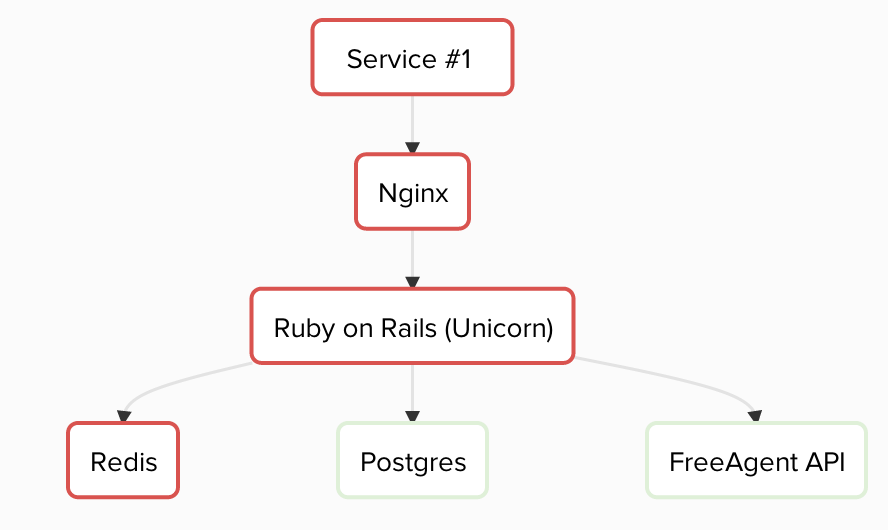
\includegraphics[scale=0.7]{web-ui/rca.png}
\end{figure}

The component `Redis' is inferred as the root-cause, as all other failing components are dependent upon it, and it does not itself have any failing dependencies.

\pagebreak
\subsection{Email and SMS Notifications}
\label{notifications}

The management API implements two methods of notification, Email and SMS. Both of these types of notification are intended to alert developers or system administrators of new incidents opened on services they are responsible for.

The email notifications are triggered when incidents open or are subsequently resolved. They provide an at-a-glance summary of the issue, together with a link to the Web UI for viewing in more detail. The emails are created via the ActionMailer functionality in Ruby on Rails and sent via the third party service SendGrid\footnote{SendGrid - http://sendgrid.com/docs/User\_Guide/index.html} via SMTP. SendGrid ensures the reliable delivery of these emails.

\begin{figure}[h]
  \centering
  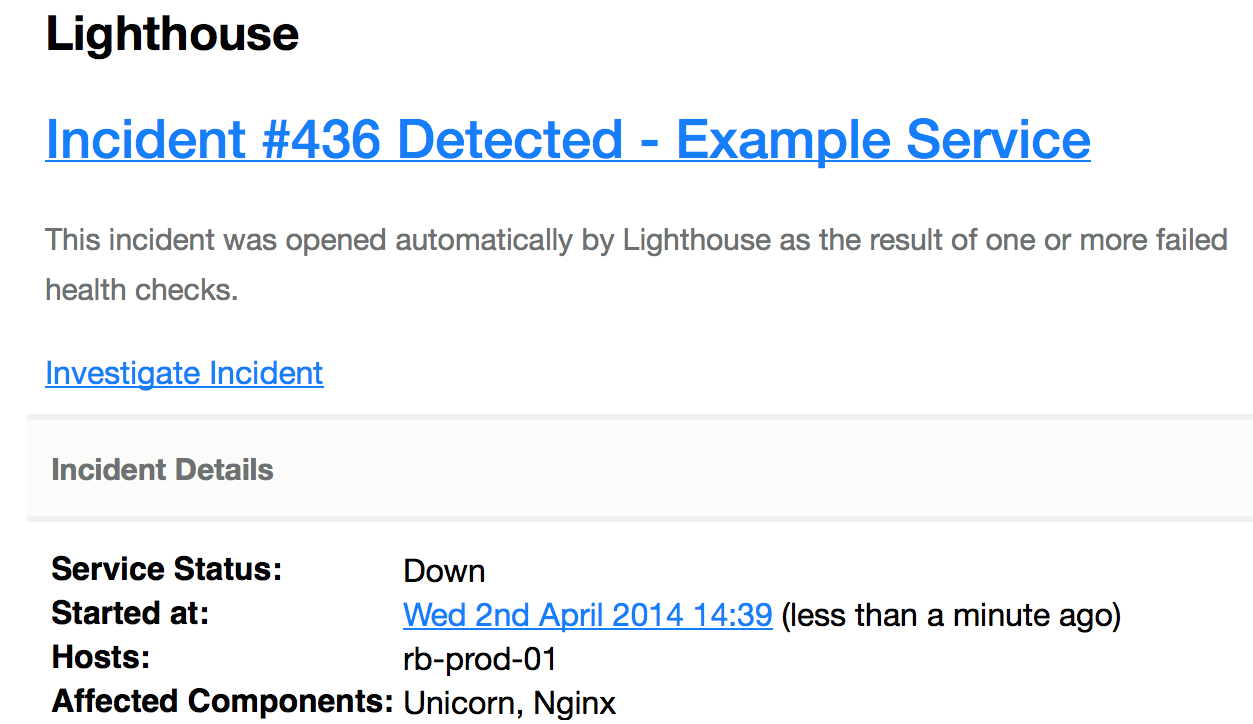
\includegraphics[scale=0.6]{email.png}
  \caption{An example email notification, triggered when an incident has been detected.}
\end{figure}

SMS notifications can convey a more limited quantity of information than emails, but can be useful when the user in question does not have access to the internet. SMS messages are sent via the third party service Twilio\footnote{Twilio - https://www.twilio.com/docs/api/rest}. Twilio provide a REST API and can deliver messages to the provided phone numbers internationally.

\pagebreak
\section{Web UI}

The Web UI is an important component, acting as the primary way for the user to visualise the state of the system. It provides a clear and simple interface to display services, components, events and incidents. Implementation choices and specific features are detailed further below.

\subsection{Implementation Choices}

\subsubsection{Traditional Website vs. Single Page Application}

The Web UI is implemented as a single page web application, written in JavaScript. Single page applications have recently increased significantly in popularity, due to the improved capabilities and performance of modern browsers. A single page application differs from a traditional website in the following ways:

\begin{description}
  \item[Rendering]
    Most web applications are executed exclusively on the server-side, this is an obvious choice as it provides many benefits such as: low-latency database access, the standard execution environment of a server under the developers control and improved security, eg.\ no direct database access or ability to modify the source code. With a single page application, the server side components are usually exposed via an API which takes advantage of these benefits, and the client-side JavaScript fetches data from this API via AJAX requests. When data is received, it is rendered into HTML elements by JavaScript executing in the browser.
  \item[Interactivity and Responsiveness]
    The user experience of a single page application can be significantly better than a traditional website, when used in an appropriate situation. Websites can feel much more like a native desktop application, with multiple views, background data synchronisation, data filtering etc. The main increase in responsiveness comes from eliminating page reloads, which incur the full latency penalty unless they are cached, thereby increasing perceived performance.
  \item[Deep Linking \& History]
    Browsers cater well to traditional web pages, as each page must have a uniquely accessible URL and is explicitly navigated to by clicking on a hyperlink. Single page applications must emulate this behaviour using JavaScript techniques to achieve deep-linking so that bookmarks or shared URL's will navigate to the correct state within an application. Features such as the HTML5 history API enable this.
  \item[Search Engine Optimisation]
    Single Page Applications are generally a poor choice where search engine rankings are important for a website. Search crawlers typically do not execute JavaScript and are therefore unable to index content effectively. For a tool such as the Monitoring UI, this is unimportant, as it is intended as an internal tool which will often be protected by a layer of authentication and not accessible from the web. Solutions for this issue are available, and involve executing the application on the server side using a JavaScript engine such as Node.js initially.
  \item[ Abstraction and Maintainability]
    Single page application frameworks often apply standard architectural patterns such as Model-View-Controller. These patterns can help to raise the level of abstraction when creating highly interactive applications beyond manually binding event listeners to Document Object Model (DOM) elements in order to update and present data. Applications that are abstracted from the imperative nature of programming with the DOM can find benefits in a more declarative approach. This can help improve testability, code reuse and can reduce the number of defects.
\end{description}

The vastly improved user experience attainable from a single page application was the primary consideration in selecting this approach. The UI is primarily read-only, but its role is to provide a near real-time view of the system from a number of different perspectives, switching between these perspectives can be seamless as a result of this implementation choice.

\subsubsection{Single Page Application Frameworks}

There are many popular Single Page Application frameworks, including: Knockout.js, Angular.js, and more recently, React.js. The frameworks vary from very small and focused (such as React.js) to the more complex and full-featured (such as Angular.js).

The Web UI is a fairly simple application, and a large framework can cause performance concerns as well as significantly increase the complexity of the code. React.js is the simplest of the mentioned frameworks, developed at Facebook and used on major sites such as Facebook, Instagram and Khan Academy, it deals with building reusable components, data binding and high performance view rendering, and its design is inspired by functional reactive programming.

React.js was chosen for this project as the simplest and most effective tool for the job, its simplicity made it extremely productive to work with.

\subsection{Features}

The Web UI is the primary method of interaction for users of the system. It provides the following main features:

\subsubsection{Getting Started Guide}

The getting started guide explains how to install and use the management agent, after the steps have been followed, the user will be able to effectively visualise the system under test.

\begin{center}
  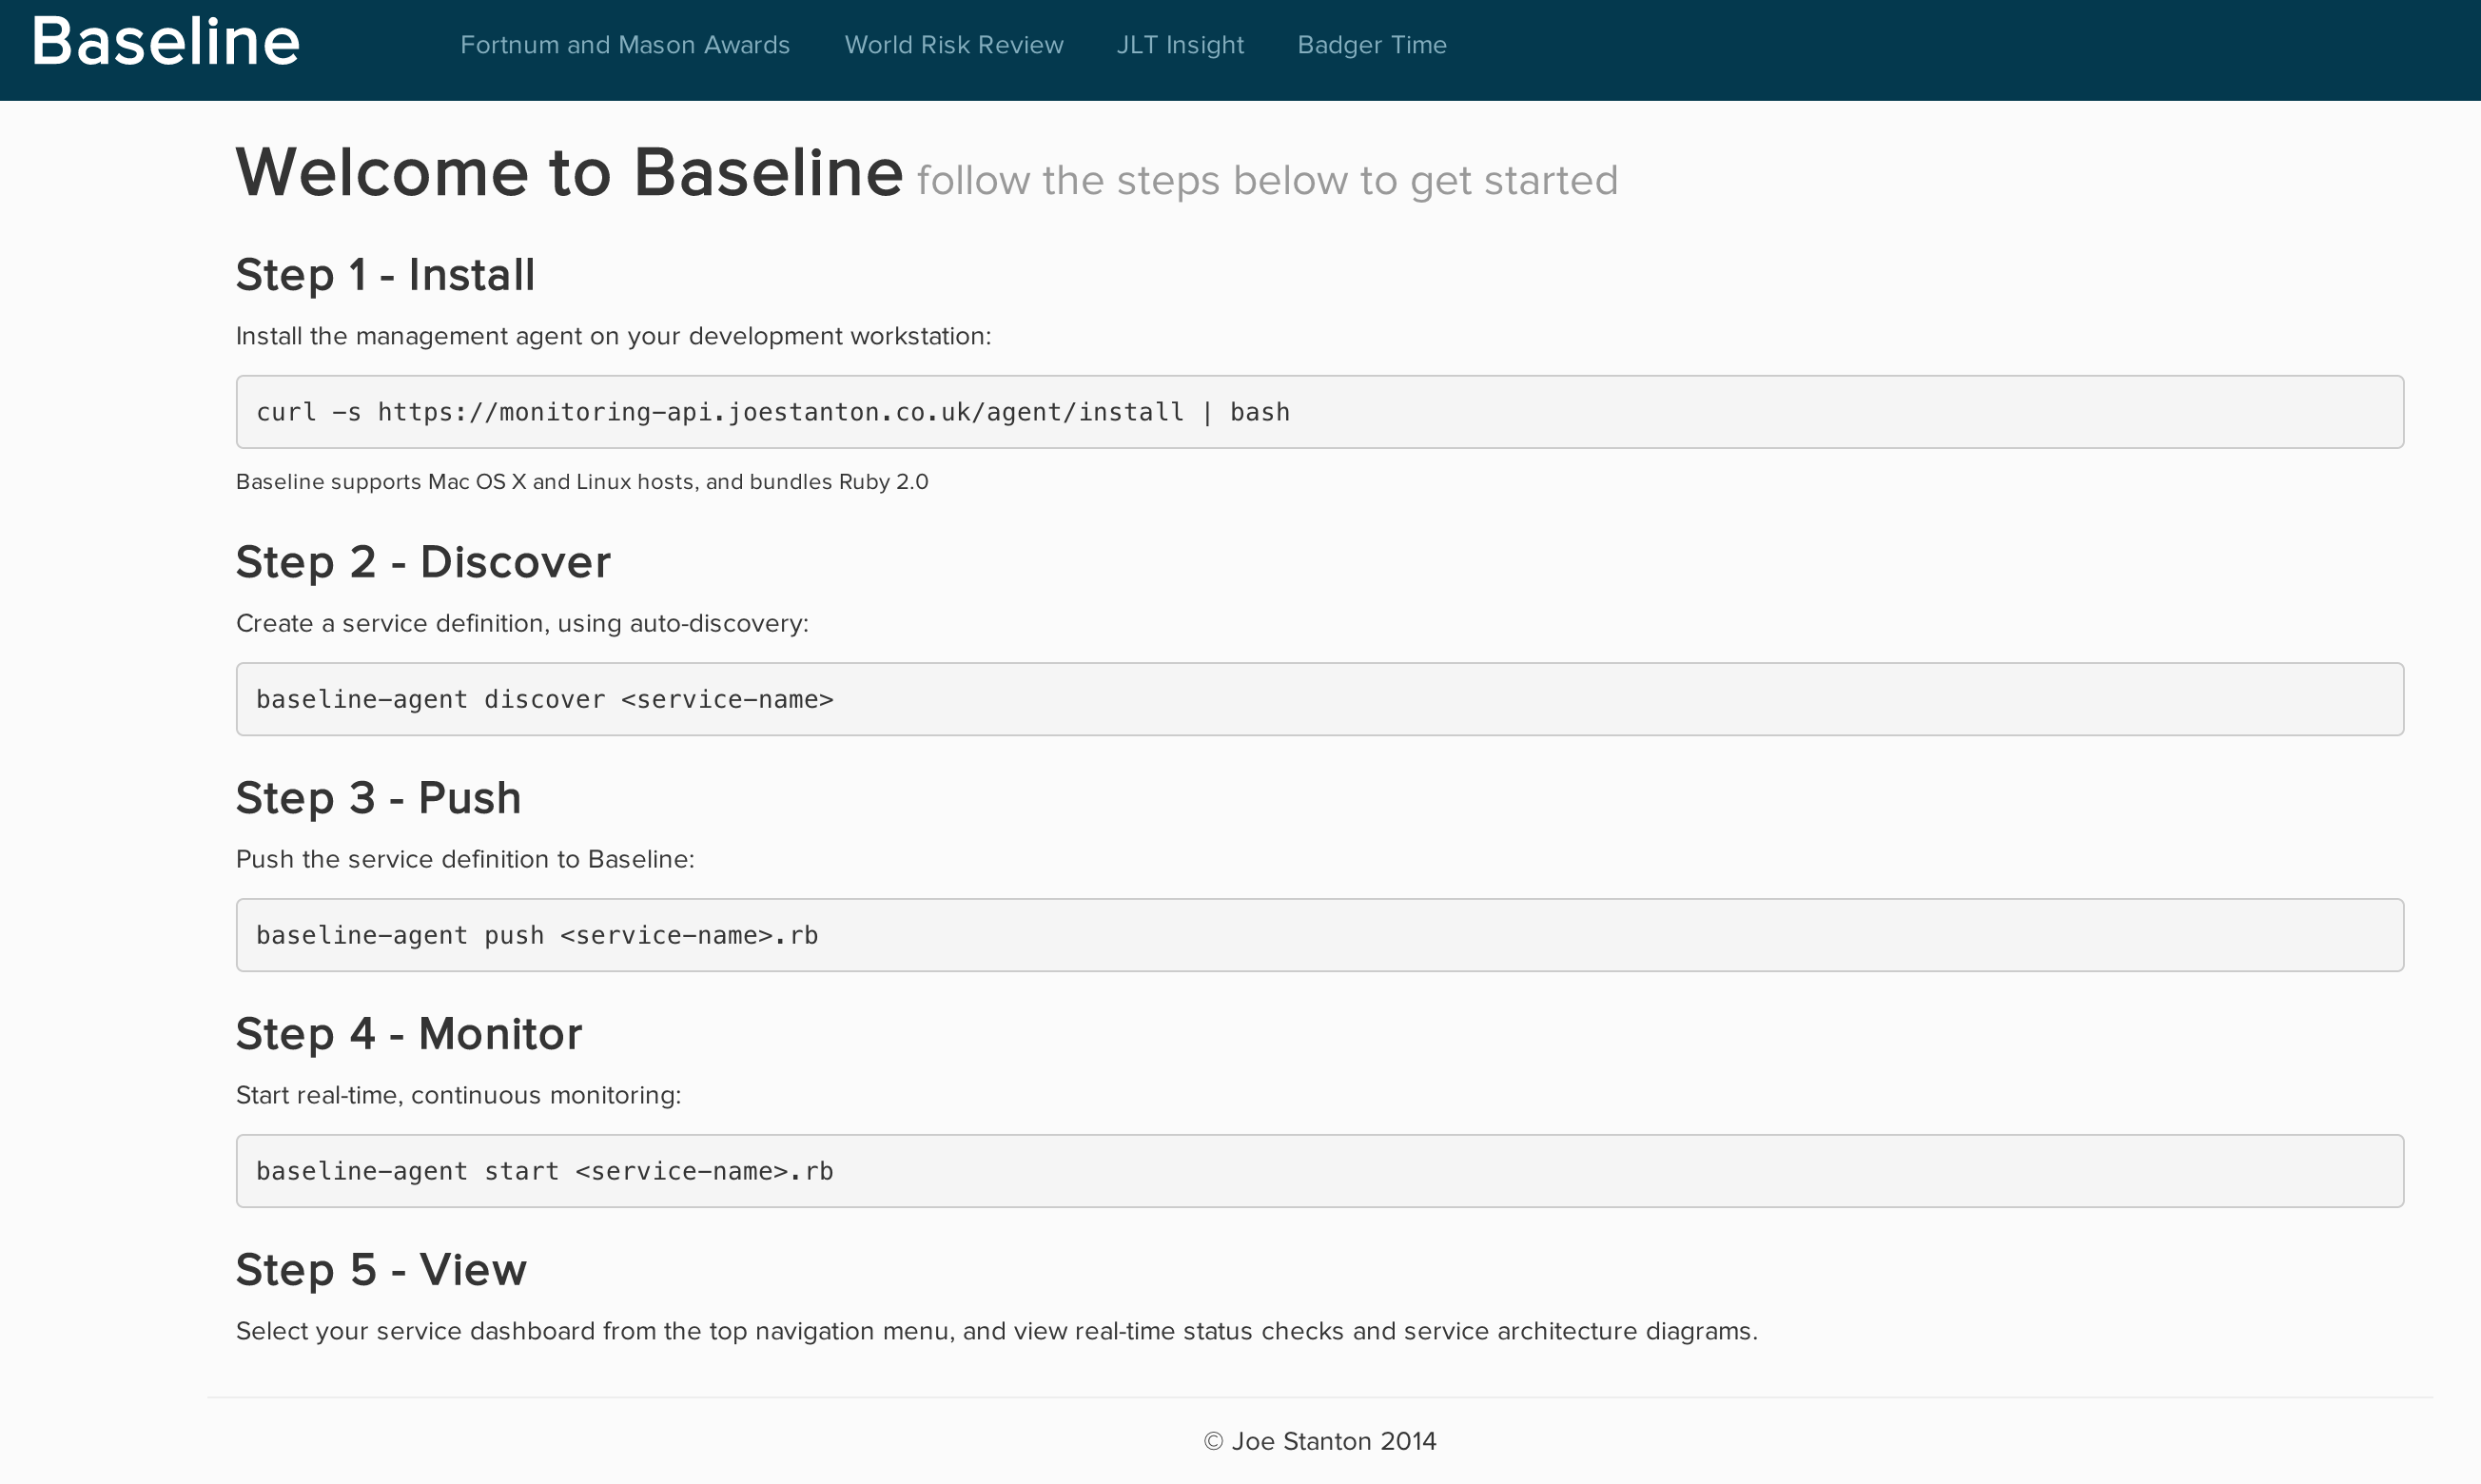
\includegraphics[scale=0.28]{web-ui/getting-started.png}
\end{center}

\subsubsection{A Service Overview}

The service overview provides the information necessary to understand the high-level architecture a service. It gives an overview of the service itself, with its description if specified, a number of reliability metrics and the current service status.

All individual components and hosts are listed, together with their respective statuses. If there are any issues within the service, they will be highlighted and enhanced with extra detail to aid in the troubleshooting process.

\begin{center}
  \label{webui-overview}
  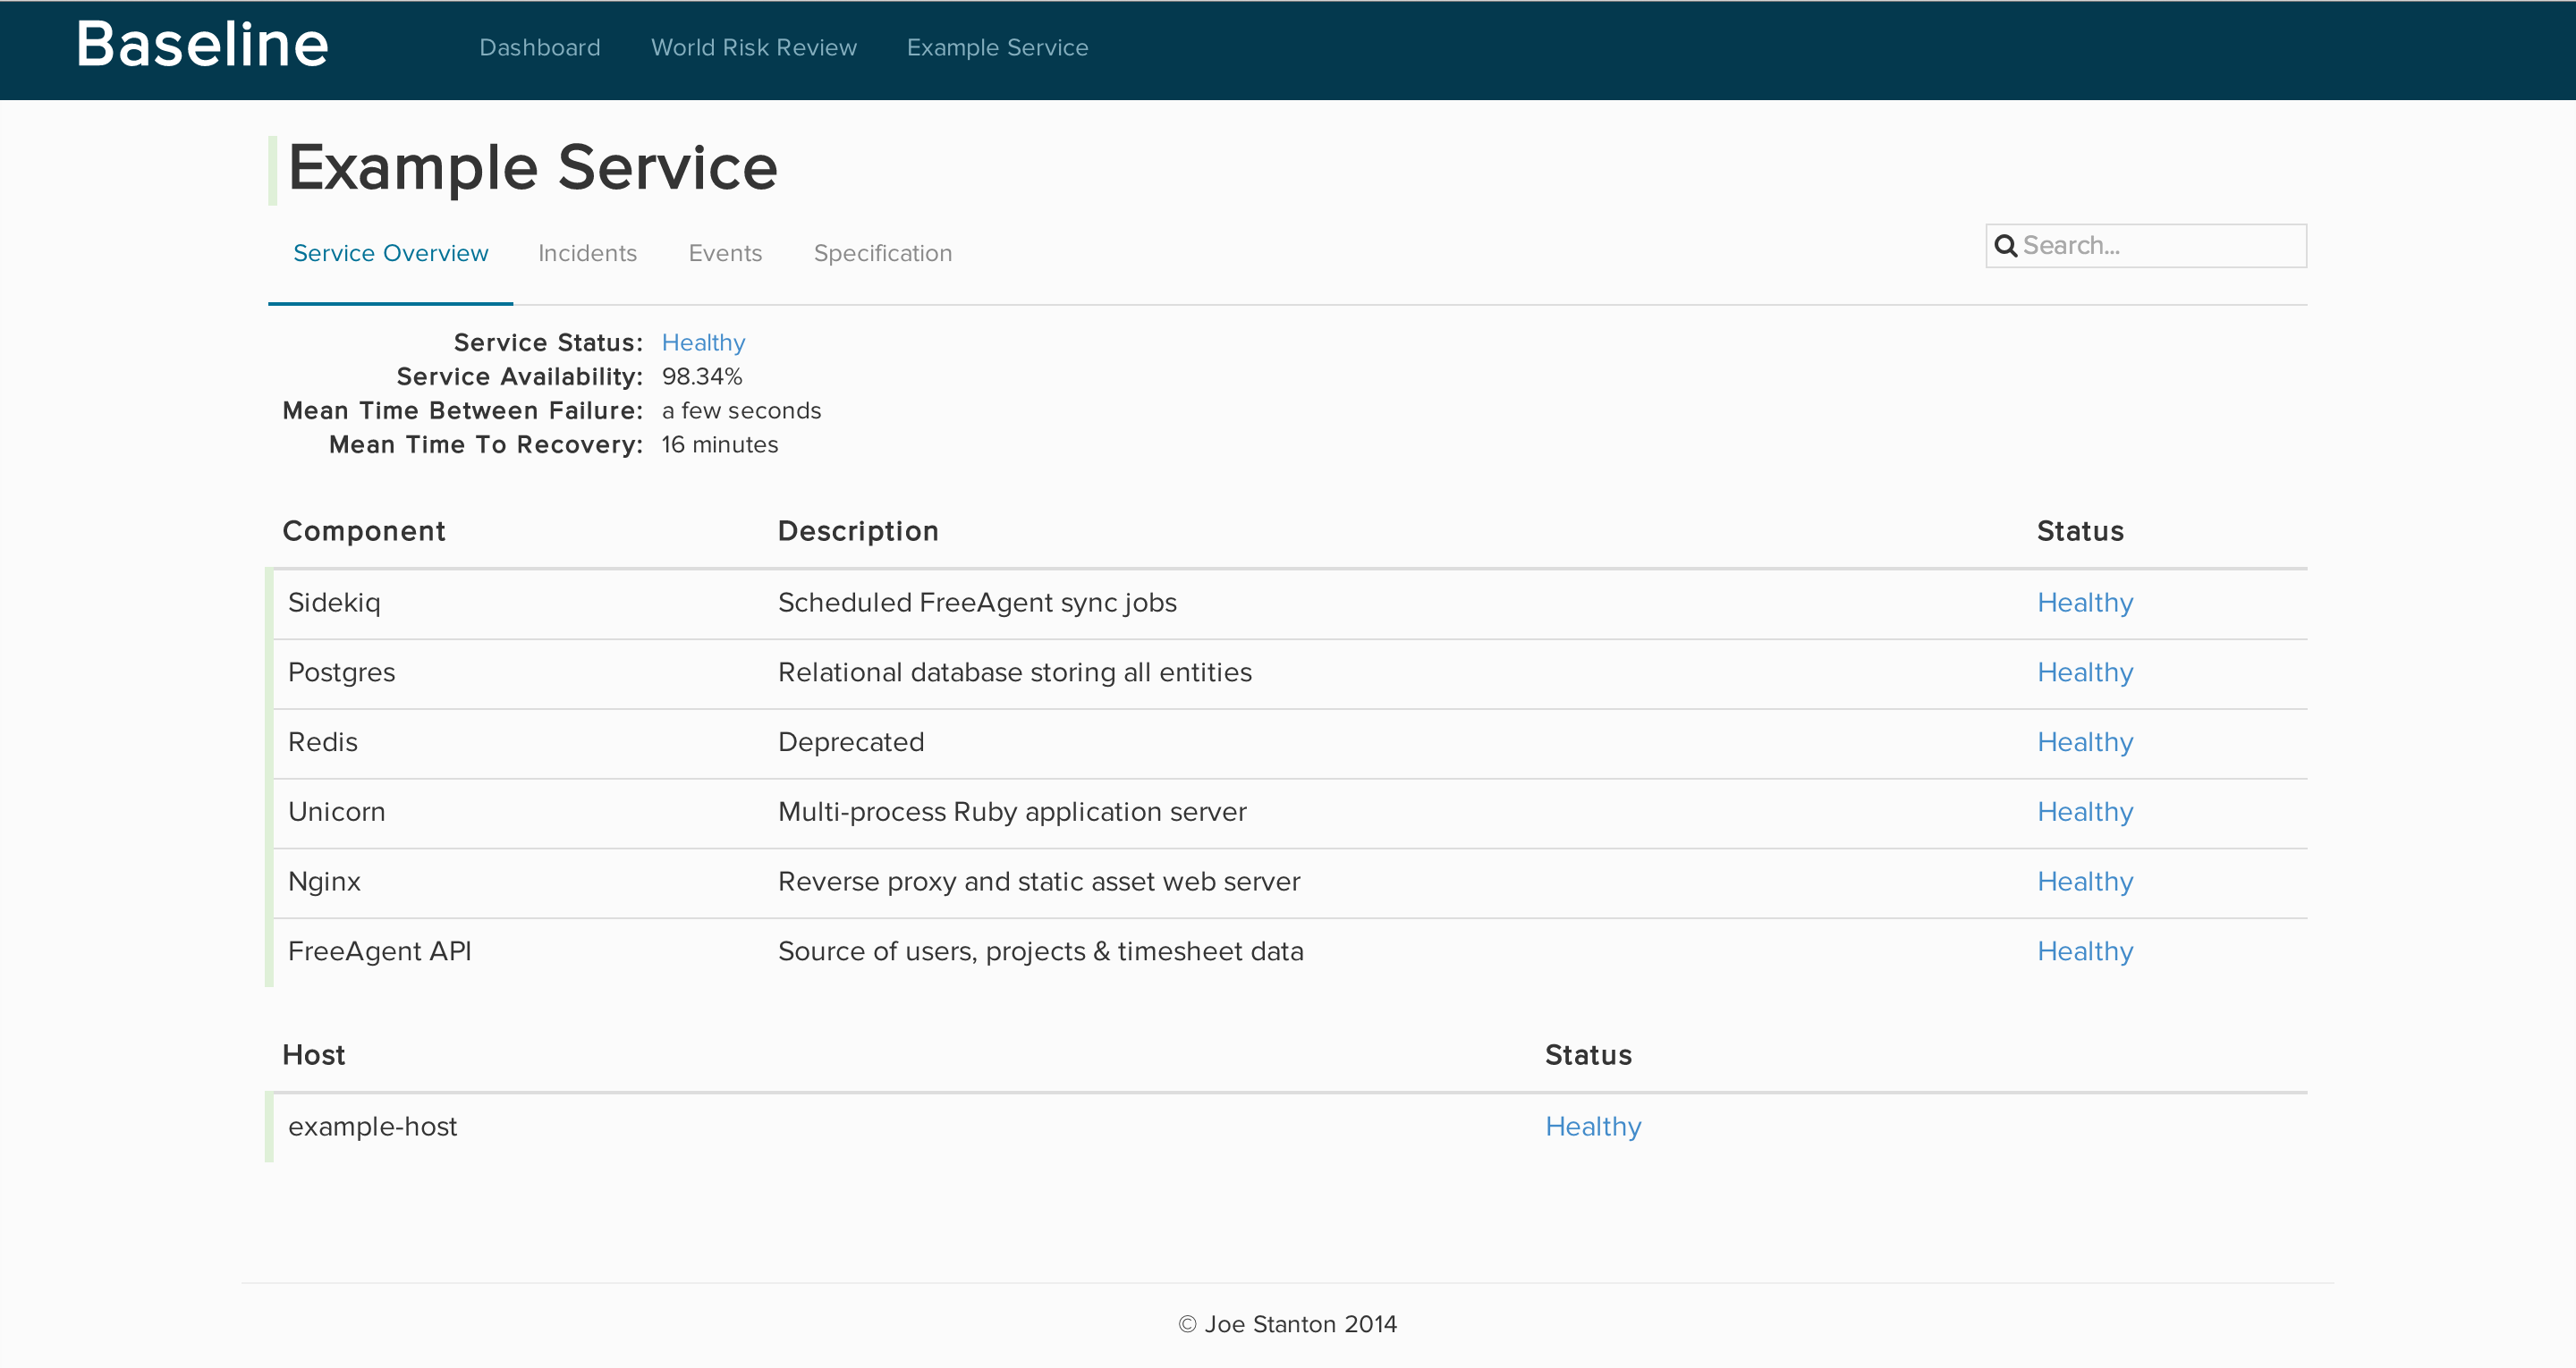
\includegraphics[scale=0.28]{web-ui/service-overview.png}
\end{center}

\subsubsection{Architecture Diagrams}

Diagrams are often the best way to express complex services with many dependencies, the Web UI uses D3.js to render Scalable Vector Graphic representations of the modelled system. These diagrams also colour code the status of each component.

\begin{center}
  \label{webui-architecture}
  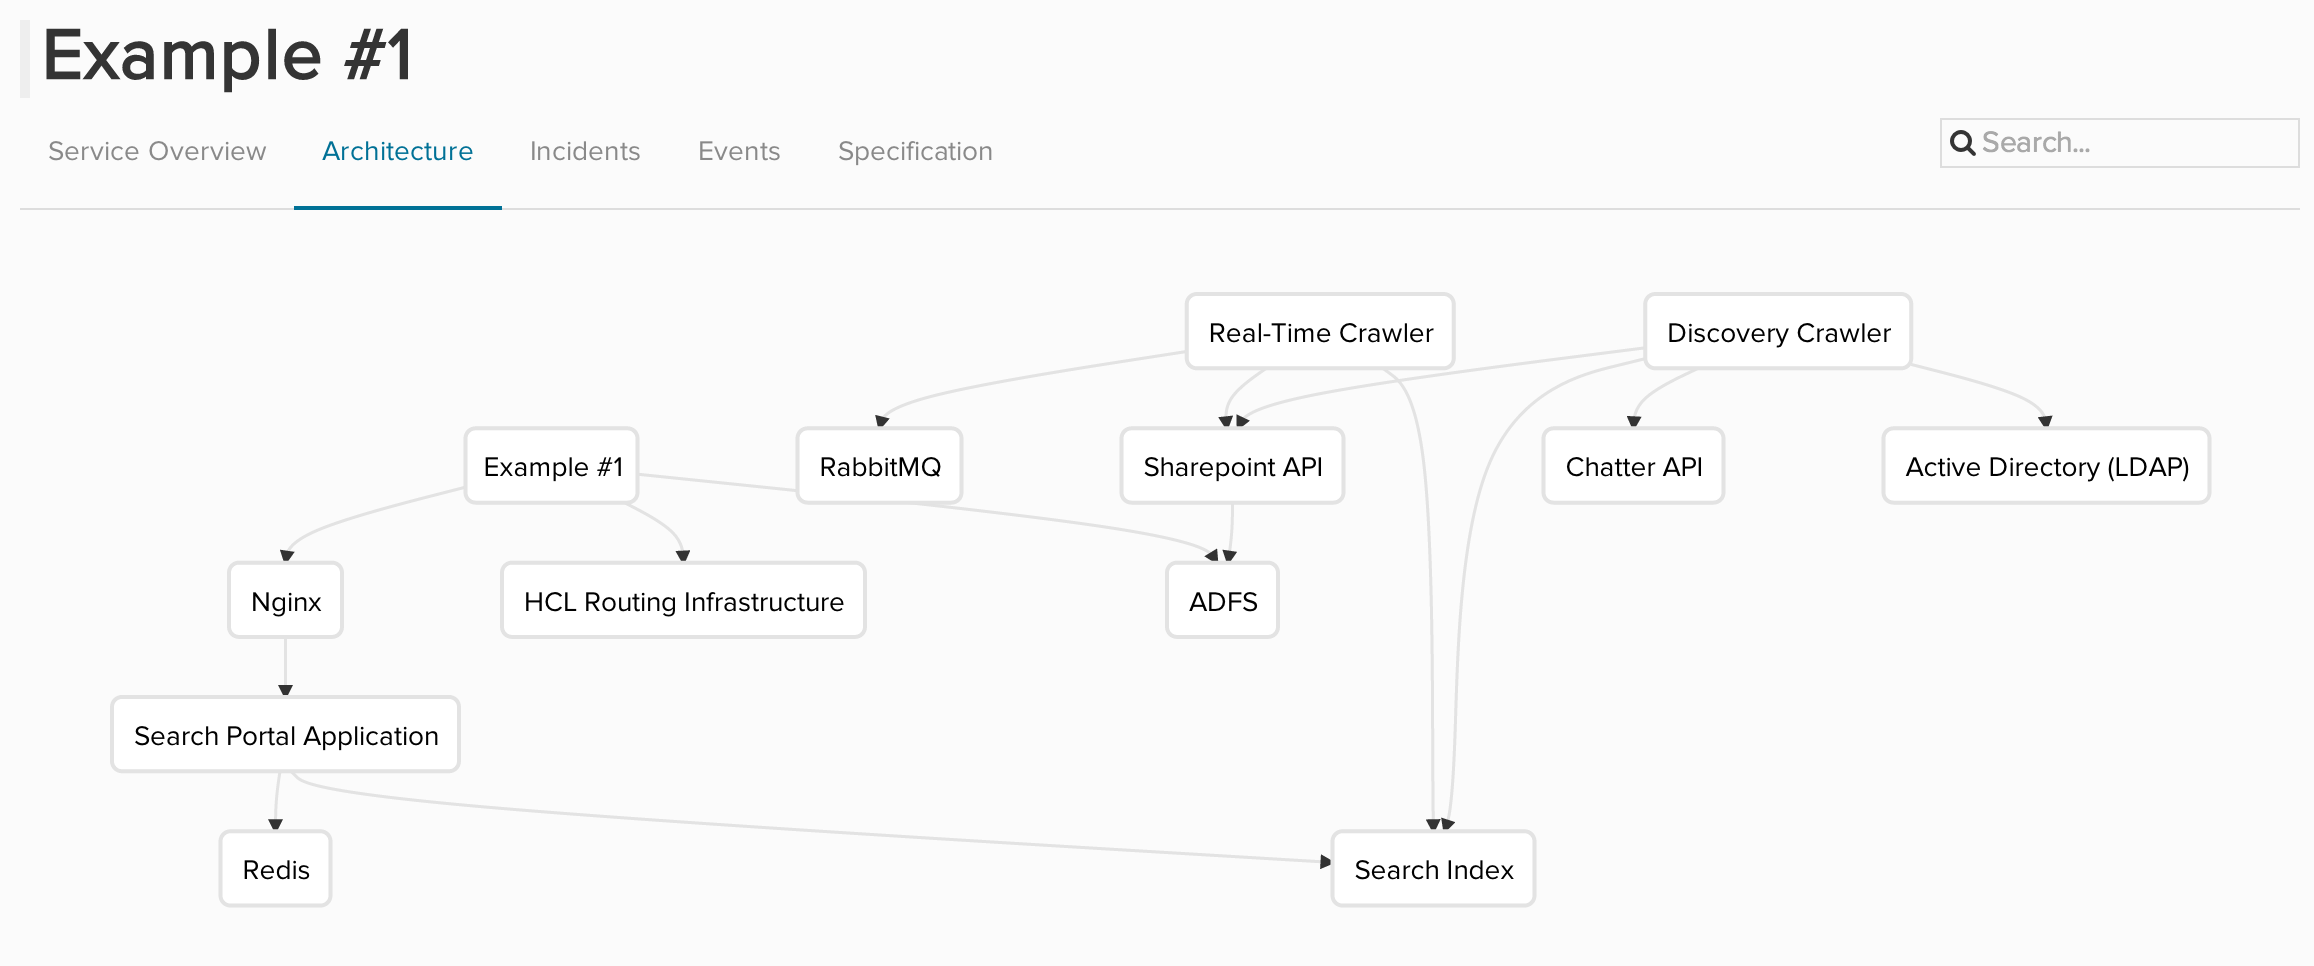
\includegraphics[scale=0.33]{web-ui/architecture.png}
\end{center}

\subsubsection{Incident Tracking}

As previously discussed, Incidents are a consolidated view of relevant context that users can use to identify the root cause of issues. Users will be directed to the incident page via notifications received via Email or SMS\@. The interface surfaces relevant events occurring before or during an incident, as well as similar incidents that have occurred in the past.

After an incident has been resolved, the user is encouraged to provide a brief note detailing the root cause, as well as any remedial action taken. This will be surfaced when other relevant incidents occur in future.

\begin{center}
  \label{webui-incidents}
  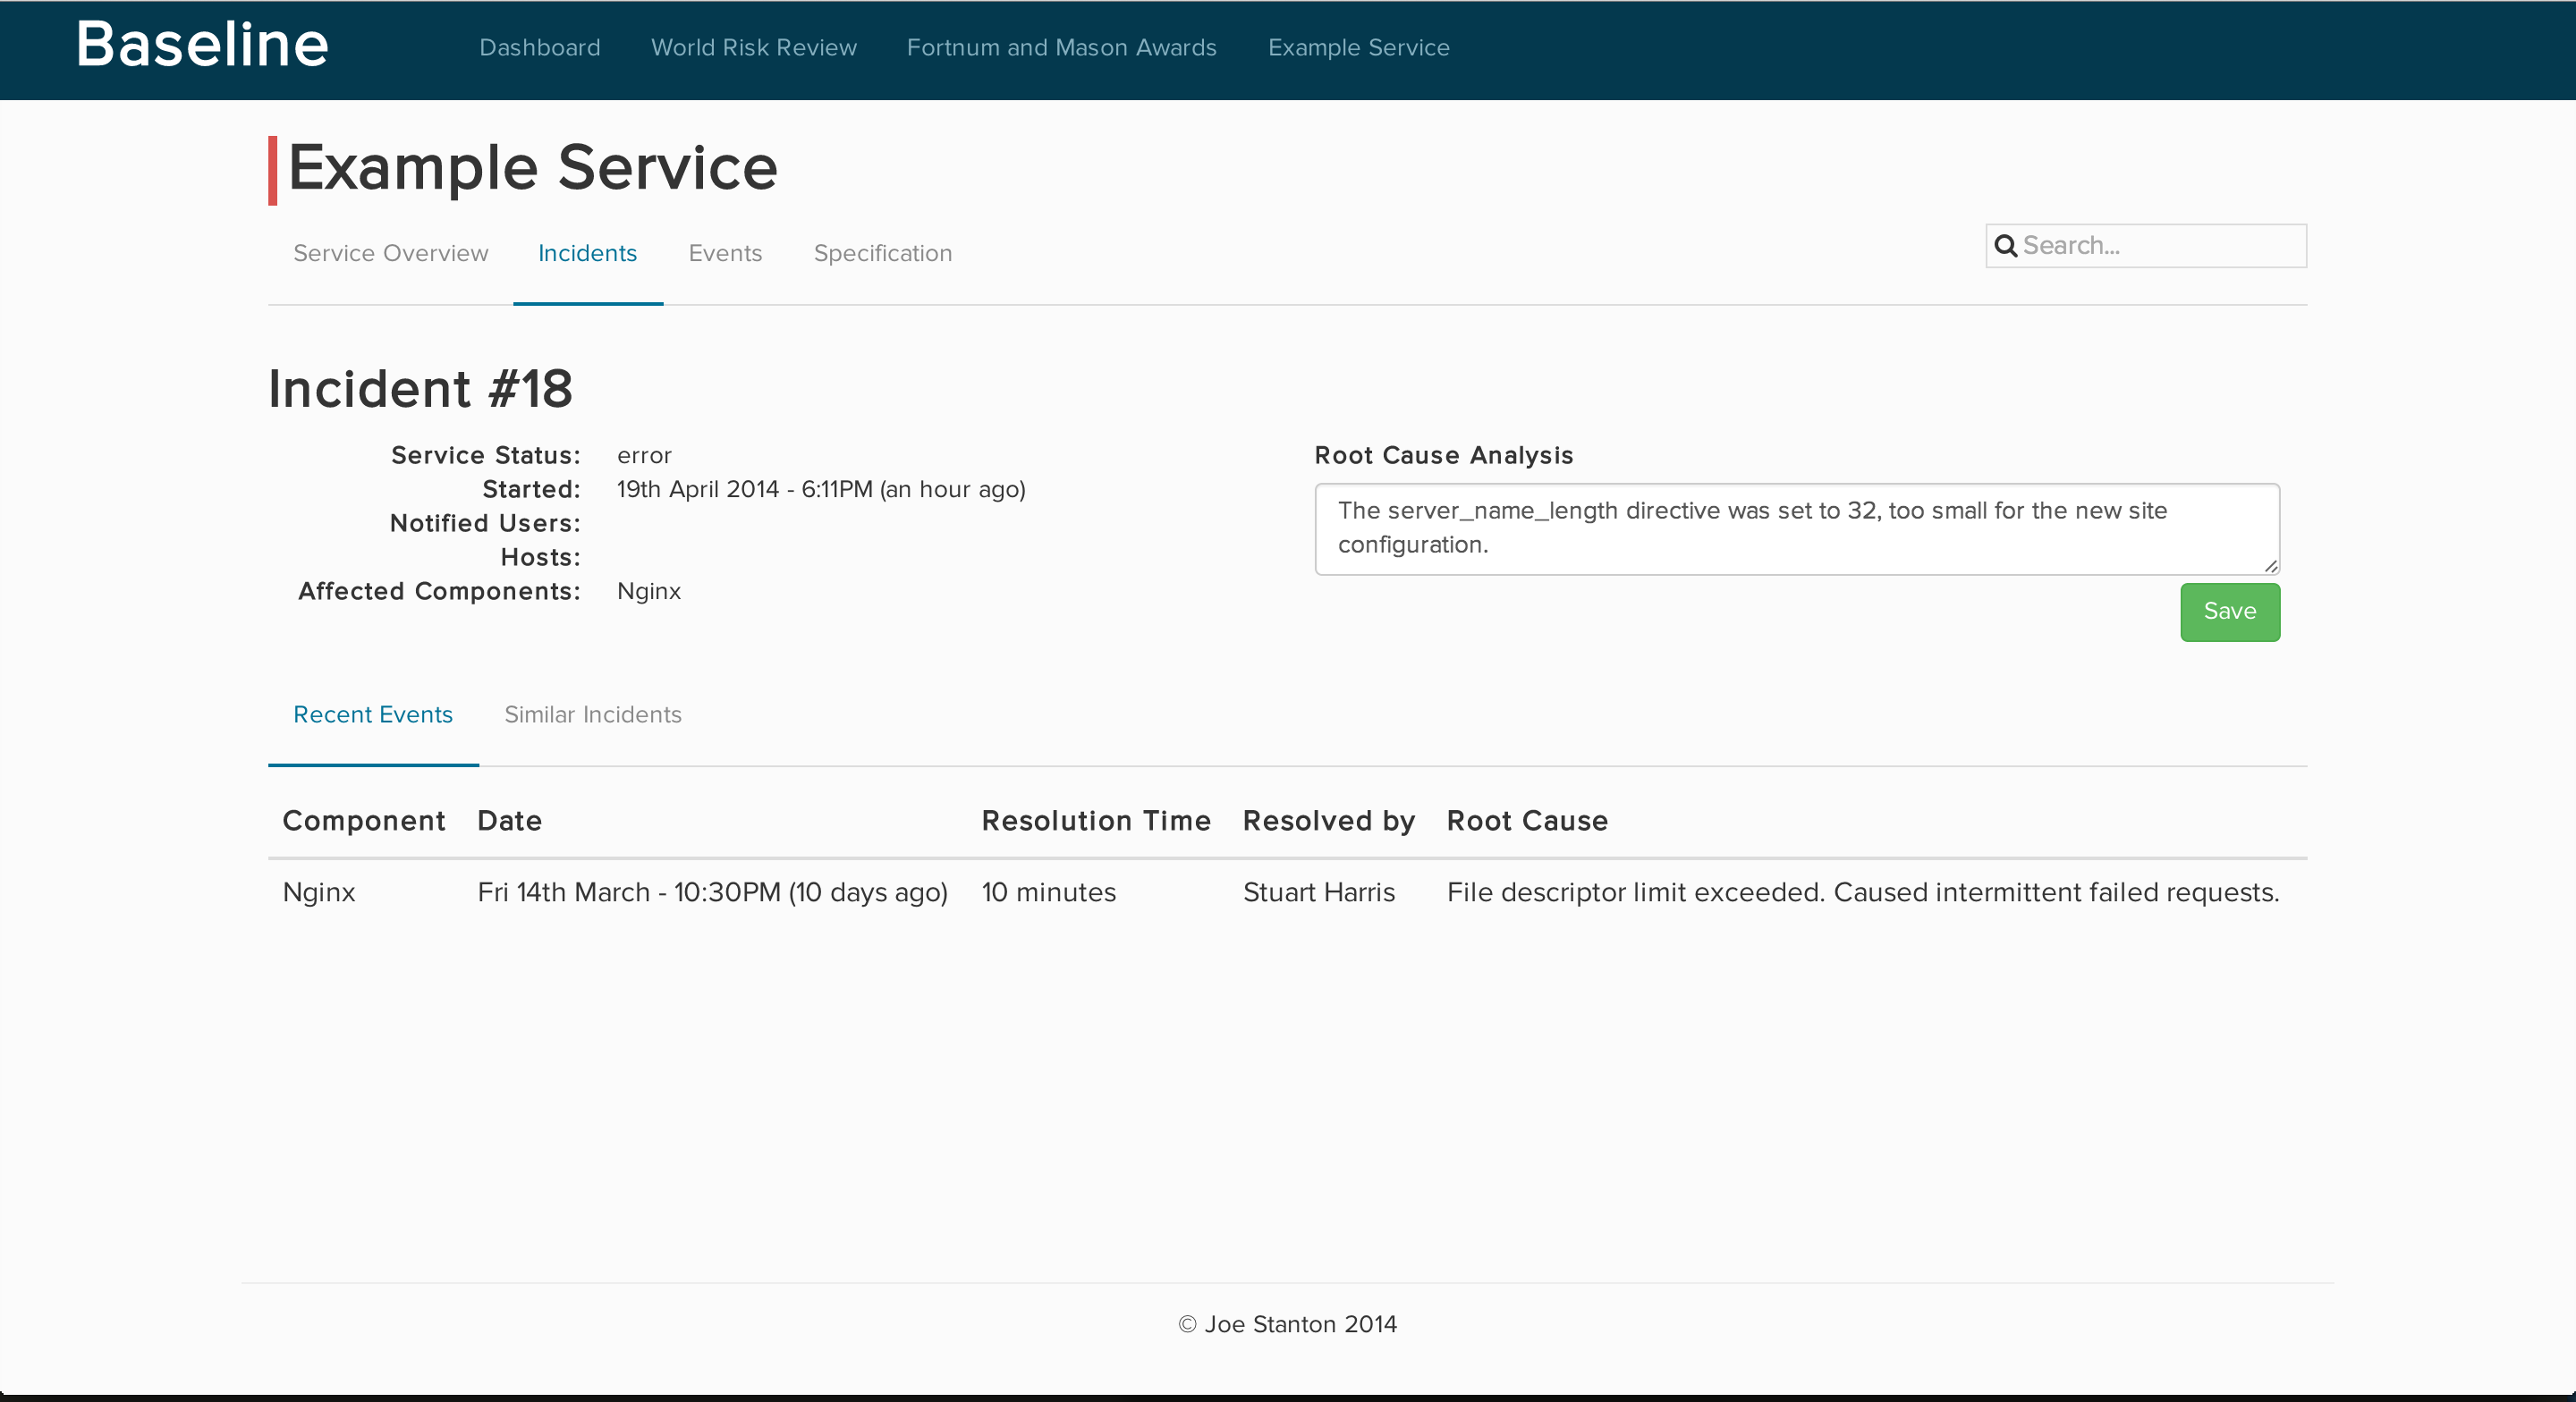
\includegraphics[scale=0.28]{web-ui/incidents.png}
\end{center}

\subsubsection{Event Logging}

The monitoring system is designed to accommodate and track changes in underlying infrastructure. The event log provides a chronological view of these changes together with supplementary information provided via each integration. For example, a deployment event will normally include meta-data such as the hosts affected, the branch deployed as well as the specific build or version number if available. The interface provides the means to filter these events, so users can easily identify changes in relevant parts of the system if issues occur.

\begin{center}
  \label{webui-events}
  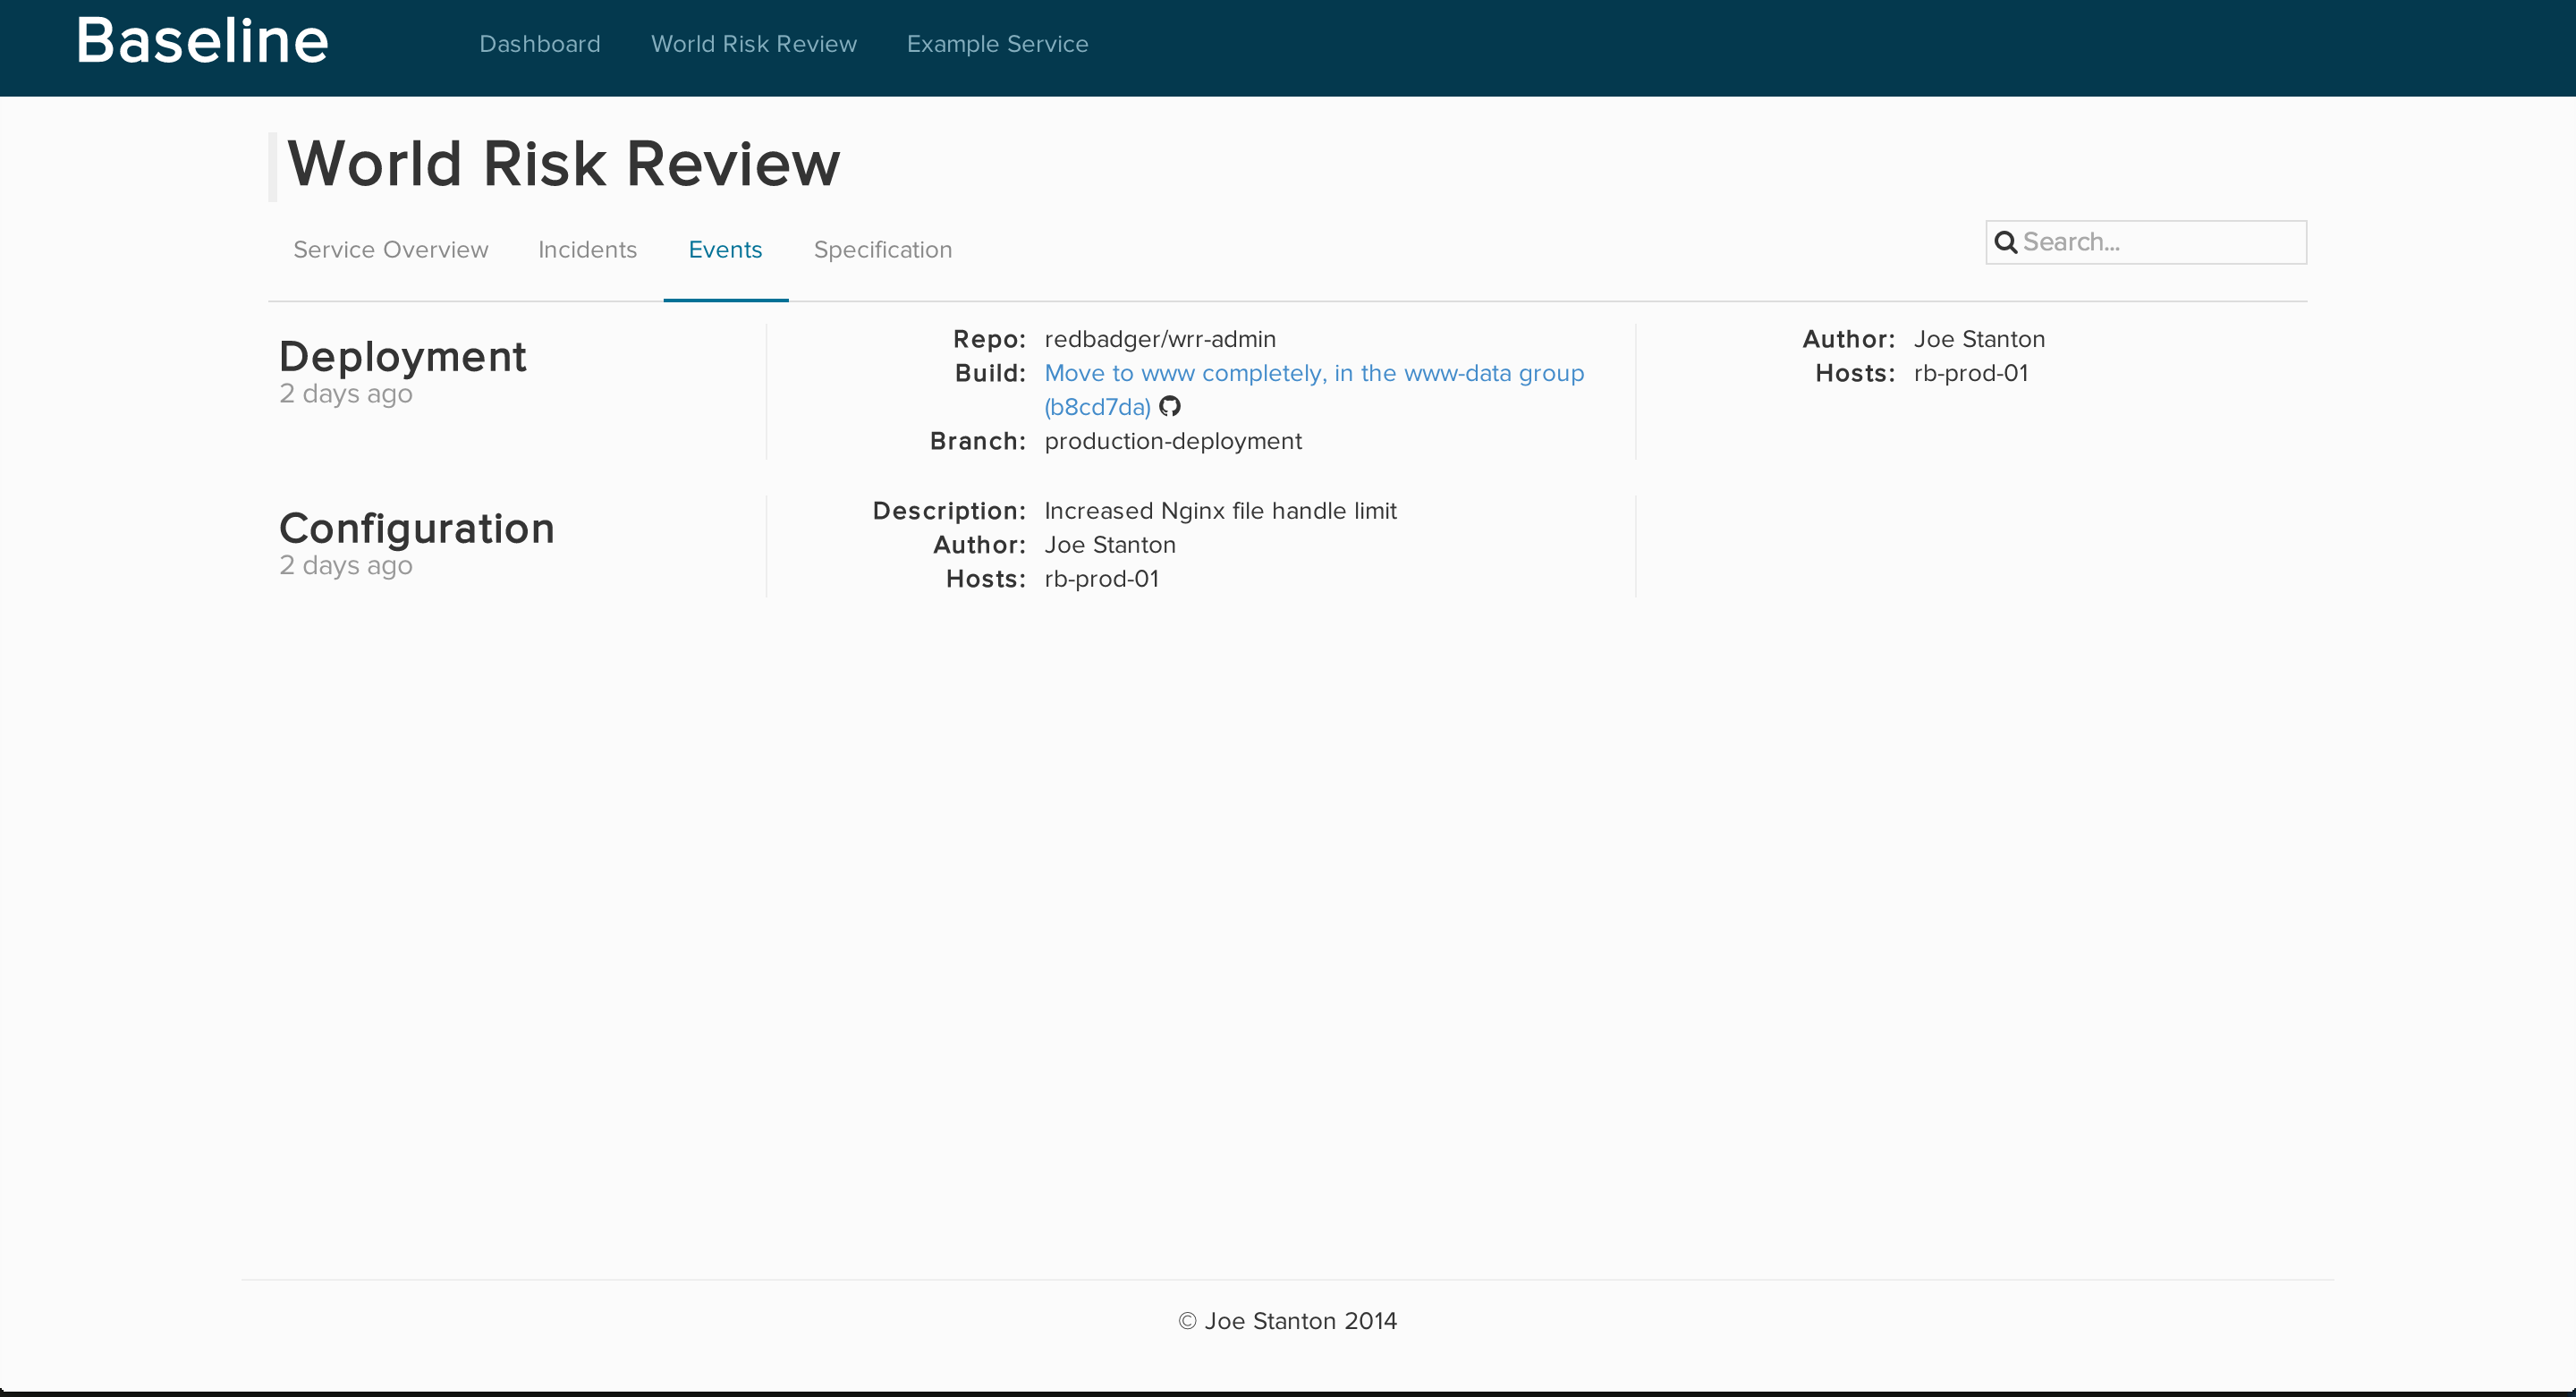
\includegraphics[scale=0.28]{web-ui/events.png}
\end{center}

\subsubsection{Specification View}
The UI provides an easy way to check the exact details of a specification, by switching to its raw representation. This is intended primarily as a debugging tool.

\begin{center}
  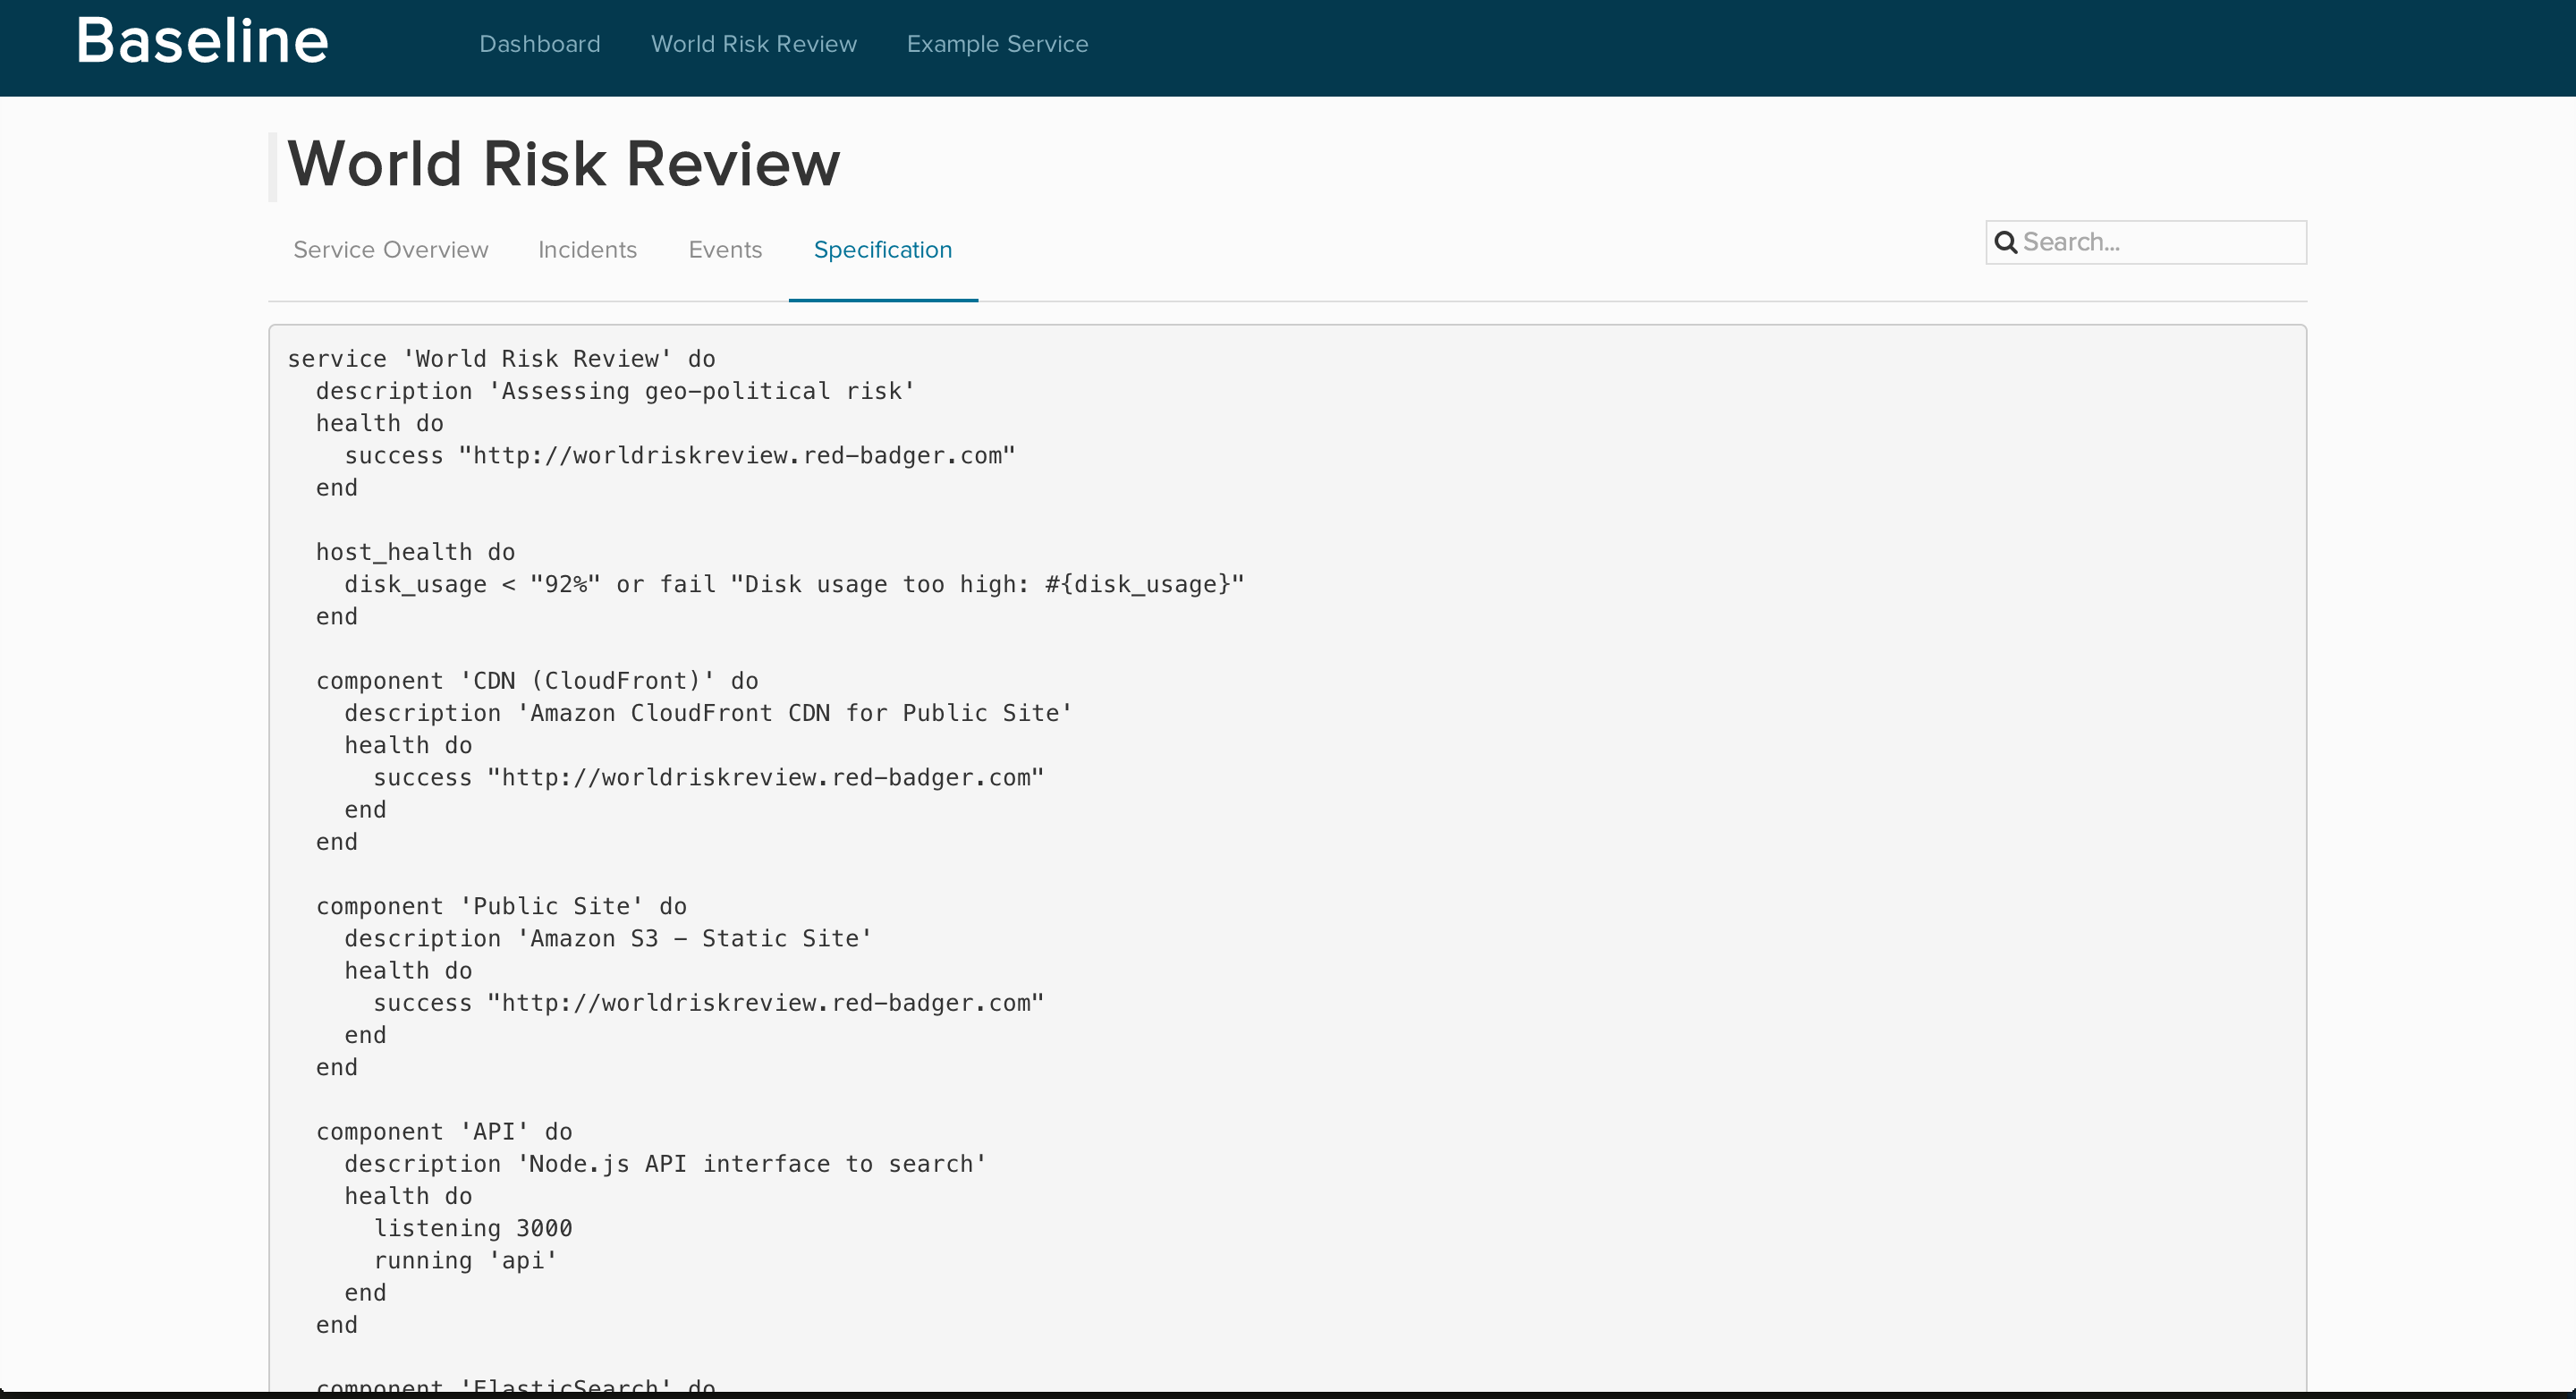
\includegraphics[scale=0.28]{web-ui/specification.png}
\end{center}

\pagebreak
\section{Deployment \& Provisioning}
\label{ansible}

The management server should have an automated, repeatable provisioning and deployment process. This involves the setup and configuration of all supporting software packages on a given host via a configuration management tool.

Automation of this process has a number of benefits: it reduces the chance of defects caused by configuration inconsistencies and can make it significantly quicker to adapt the infrastructure in future. Most significantly, it will make it simple to package the tool as a virtual appliance or provision a bare-metal machine that can be deployed on a user's private network. This will become the `on-premise' version of the tool, more suitable where there are a large number of checks or the system under test stores sensitive data. A hosted version of the tool may also be provided.

\subsection{Configuration Management Tools}

As discussed in the background research section, configuration management tools allow the specification and configuration of software packages on any number of hosts. They are most useful when dealing with a large number of nodes or where there is a need to generate whole machine images as part of a build process. A configuration management tool normally executes a set of scripts idempotently to check and enforce convergence with the specification.

\subsubsection{Ansible}

Ansible is one of the simplest configuration management tools around. Its competitors, Chef and Puppet, provide significantly more functionality that is not required for this project. Many of the features of Chef and Puppet allow them to efficiently orchestrate changes on large numbers of hosts, and offer more features for platform agnosticism, this carries some extra complexity. Ansible is a simpler variant more suitable for a small number of nodes, and its simplicity makes writing ``playbooks" quick and painless.

Ansible ``playbooks" are declared in YAML format. Ansible contains specific modules for most types of configuration task, usually implemented as thin wrappers around UNIX commands. It builds in checks to ensure that commands are idempotent. This allows the user to repeatedly use a playbook with no negative effects on the host. The playbooks look similar to the following:

\begin{listing}[p]
\begin{minted}[fontfamily=fi4]{yaml}
- name: Install Dependencies
  apt: pkg={{item}}
  with_items:
    - python-software-properties
    - software-properties-common
    - python-pycurl
  sudo: yes
  tags: nginx

- name: Add Nginx Repository
  apt_repository: repo=ppa:nginx/stable
  sudo: yes
  tags: nginx

- name: Install Nginx
  apt: pkg=nginx-full
  sudo: yes
  tags: nginx

- name: Configure Nginx
  template: src=nginx.conf.j2 dest=/etc/nginx/conf.d/default.conf
  sudo: yes
  tags: nginx

- name: Set /var/www/ permissions
  file: path=/var/www/ mode=0644 state=directory
  sudo: yes
  tags: nginx

- name: Start Nginx
  action: service name=nginx state=restarted
  sudo: yes
  tags: nginx
\end{minted}
\end{listing}

\subsection{Virtual Appliances - Packer}

Packer is a tool that creates machine images from a given hardware specification from scratch. It integrates directly with configuration management tools such as Ansible to prepare the machine image after it has been created. Packer builds the following machine image formats:

\begin{itemize}
  \item Amazon Machine Images - Used widely on Amazon AWS, these images specify the hardware specifications of a virtual instance, together with a pre-prepared filesystem. These images can be used directly to boot a virtual instance into an existing AWS account with a single click.
  \item Open Virtualization Format (OVF) - Supporting VMWare and VirtualBox, this format can be used to directly import an appliance to VMWare ESXi or other enterprise virtualization platform. Test instances can also be booted on a development workstation.
\end{itemize}

A configuration file controls the setup of a base Ubuntu Linux v13.04 image, Packer then executes the Ansible playbooks before exporting the image to the specified formats. The convenient packaging of the software should increase the chances of adoption significantly.

\pagebreak
\section{Tools and Methodologies}
\begin{description}
  \item [Version Control]\hfill \\
    Due to the size of the project and significant development effort involved, \textbf{Git} has been used to version control my codebase. The code itself is distributed across 5 separate repositories. It is hosted as a set of open-source repositories at \textbf{GitHub} for redundancy and issue tracking features.

  \item [Test Driven Development]\hfill \\
    It is of utmost importance to ensure that the codebase of the monitoring tool is as free from defects as possible. An unreliable monitoring tool eliminates all of the safety guarantees a stable tool would provide. As further detailed in the testing section, Test Driven Development has been extensively used to verify the correctness of each component as it is implemented.

    Where this is particularly difficult due to a large number of side effects or dependencies, slower integration testing was used to provide some high-level guarantees and ensure that the system satisfies its requirements. A small amount of manual testing was also required.
  \item [Vagrant and Amazon AWS]\hfill \\
    Where integration tests are required, Vagrant\footnote{See
    https://docs.vagrantup.com/v2/why-vagrant/index.html - Benefits of using Vagrant} is used.Vagrant is a Ruby scripting tool that controls
    VirtualBox\footnote{See https://www.virtualbox.org/ for an overview of VirtualBox} and automates the provisioning and setup of Virtual Machines according to a specification.

    These provisioned virtual machines have been used to test cross-platform compatibility of the solution, and to simulate failures and verify the behaviour of the monitoring tool.
\end{description}

\pagebreak
\chapter{Professional Issues}

As this tool is designed to be deployed and used in a professional environment, there are a number of issues I have taken into consideration, these include:

\section{Plagarism \& Licensing}
    The delivered solution makes use of a number of open-source libraries and tools, such as the Riemann event processor, Ruby on Rails and a number of common RubyGems. The delineation between my own work and that of others has been made clear throughout my report, it will also be documented in developer notes.

    Many of these libraries have different licenses, but all permit usage within commercial software. As my tool is also open source, a number of licensing implications do not apply, but if a commercial offering was made in future, these would have to be reconsidered carefully.

\section{Developer Competence \& Risk}
    The codebase has been made open-source to encourage audits and improvements from more experienced developers. This should help to to uncover and rectify any significant defects which could affect the tools functionality in a live environment.

    Additionally, no bold claims about the tools maturity or stability will be made in the documentation without significant prior evidence. This should ensure that any adopters of the tool are able to make a well informed decision about any risks involved.

    As the tool runs in its own process, and background processing happens on a separate server, ideally it should not directly cause the failure of other components, but side effects such as extremely high resource/bandwidth usage could have a negative impact on live services. Wherever possible, best practices such as unit testing and rigorous functional testing have been used, and development has been carried out diligently with these issues in mind. The testing phase revealed no such issues of this nature.
\section{Data Integrity \& Security}
    The tool will be installed onto servers which will likely contain sensitive data. Therefore it is essential that precautions are taken to prevent the leakage of this data resulting from the use of this tool. This issue was considered extensively during the design phase, and has resulted in an architecture in which it is not necessary for the management agent to listen on a network interface, or require the opening of network ports upon a firewall. The tool is self-hosting within a private network if desired, where it typically will be isolated from external networks via a firewall, and subject to any company specific security policies. This means that the attack surface area for a given service is not increased by using the tool.

    Secondly, the installation and subsequent communication between the management API and system under test is encrypted via HTTPS/TLS\@. If a malicious third-party was to intercept or redirect the monitoring traffic within a private network, the data would not be readable without the server's private key, this also prevents tampering by a proxy.

    Thirdly, the tool is not yet available as a ``Software as a Service' offering, but if this is pursued at a later date, each instance of the tool must be isolated from the other, so as to avoid any leaking of data between users. Generally, it may be safer to run many instances of the application using virtualization, so as to be sufficiently isolated from other users.

\chapter{Testing}

Testing is an extremely important part of the software development lifecycle, and is key to delivering a quality product. The system I have developed composes a number of interconnected components, each of which must be tested in isolation and as a whole, to ensure correctness.

A number of strategies were chosen to test the application, detailed below.

\section{Unit Testing}

Unit Testing is a simple and effective way of ensuring units of functionality such as classes and methods behave correctly. Unit testing can be used to pinpoint the exact cause of a problem, as the code tested is isolated as well as possible from other interacting components such as databases. Running tests frequently during development provides a fast feedback loop in which correctness of new code can be verified, as well as detecting unexpected regressions in other areas of the code.

Both the API and Management Agent were developed using Test Driven Development, this is a development methodology which involves writing failing test cases before the implementation code. By writing tests as a natural part of the development process, a high amount of code coverage can be achieved without significant extra effort. Both of these components have strong unit test suites which were invaluable during the development process and beyond.

The management agent in particular benefited from this form of testing. The DSL uses a number of meta-programming capabilities of Ruby, discussed in a previous section. The meta-programming features can, in some cases, make it harder to reason about the correctness of the implementation. A suite of unit tests specifically for the parsing of the DSL were both simple to write and extremely valuable in improving its quality and correctness.

The small amount of configuration within the event streaming service was also unit tested. As Riemann itself is a well tested event processing library, there was no need to test its functionality too. Therefore there are only a couple of test cases needed for this component.

The Web UI was not unit tested. The Web UI primarily fetches and presents data to the user and the layout of this data changed significantly during the course of development. Unit testing the UI would have lead to very brittle test cases, which would break with any minor change. A combination of functional and manual testing were deemed to be a better fit for this component.

\section{Functional Testing}

While unit testing can be very beneficial in improving the quality of individual components, it does not expose any defects relating to the integration of these components into the whole system. Functional tests can vary from the combination of two components to testing the entire system end-to-end in order to validate if requirements have been satisfied.

Functional tests can typically be automated in the same way as unit tests, but it is generally more challenging and time consuming to do so. They can expose a large number of more subtle defects which are much more difficult to find after the software has been deployed.

The end-to-end monitoring process, from parsing a service specification to displaying its results on the Web UI, requires the orchestration of a number of components, some of which are distributed over the network.

Below are examples of the functional tests carried out, as they correspond to an important piece of functionality that is not possible to verify via unit tests:

\begin{itemize}
  \item When a host is setup via the installation script, it should appear on the admin interface with the correct hostname, port and service.
  \item When agent service discovery is executed, each service listed within the agent service definitions should be detected.
  \item When a service specification is pushed to the management server, it should appear on the web interface with the correct name, description and set of components.
  \item When the monitoring agent is running, it should send events of the correct format back to the event stream at the configured polling interval.
  \item When the state of a service, component or host changes, an incident email alert should be received by all appropriate users. (Automated \& Manual Verification)
  \item When a host stops sending events due to connectivity problems or a management agent defect, an incident email alert should be triggered.
  \item Subsequent failures for the same service should be grouped into a single incident. (Automated \& Manual Verification)
  \item Third party services should be able to add events to the API. (Automated \& Manual Verification)
\end{itemize}

%\section{Performance Benchmarking}
%\label{performance}
\section{Real World Usage}

Since approximately half way through the development process, a prototype of the system has been running on a number of production servers. These servers were supporting real services and the system was acting as the primary mechanism of detecting failure. This form of testing has been the most valuable. A number of minor issues could only be highlighted when the tool had been fully distributed across the internet, and others emerged after many days of continuous operation. Where problems were identified, they were reproduced with a unit test and subsequently fixed.

Some positive findings from real world usage testing include:

\begin{itemize}
  \item It was simple to write a basic set of tests for an existing service.
  \item The produced architecture diagrams were invaluable in checking the accuracy of a service specification, as well as communicating this to others.
  \item The service discovery feature was simple and effective, and provided a usable service specification template to build upon.
  \item After the initial setup, it became obvious that the tool could be used to detect some subtle problems, such as missing nightly database backups.
\end{itemize}

Results of this testing highlighted the following issues:

\begin{itemize}
  \item A large number of events accumulated within the system, causing a significant delay when loading the Web UI. Some problematic checks were fixed, and the amount of data returned from the API significantly reduced, fixing the problem completely.
  \item Connectivity issues between the host and the management API are quite common, often only lasting for a few seconds. The main solution to this was to increase the time window before a previous event had been declared ``expired". Setting the event validity period to approximately 3 times the check interval allows for up to three consecutive lost packets, more indicative of a real problem.
  \item The number of alerts produced is inversely proportional to their value. If alerts are triggered with zero tolerance for failures, the system administrator is unreasonably burdened with issues which will resolve themselves in a few minutes. This results in failures being ignored, or the disabling of checks completely. Incidents now trigger after a short delay, increasing the confidence in a real problem and collecting extra information before alerting the system administrator.
\end{itemize}

\chapter{Evaluation}

The following chapter will provide a critical analysis into the delivered solution. The function and non-functional requirements specified at the start of the project will be used as the basis for this evaluation.

\section{Functional Requirements}
\newcommand\litem[1]{\vspace{0.2cm} \item #1 \vspace{0.2cm}}
  \begin{enumerate}
    \item Testing Framework
    \begin{enumerate}
        \litem{The developer should be able to install the tool on their development workstation and servers.}

        This requirement was satisfied. The installation process was tested on each target platform, Linux (Both Ubuntu 13.04 and Red Hat Enterprise Linux 6) and Mac OS X. A single command as documented in \autoref{bashinstall} provides this functionality on all target platforms.

        \litem{The developer should be able to use to the tool to describe a system accurately and concisely.}

        A number of production systems were described using the service specification DSL, all components could be represented accurately and concisely, examples can be found in \autoref{dslexamples}.

      \litem{The developer should be able to execute this description to validate the correctness of a system, verifying any arbitrary property as required.}

        Service specifications, such as the examples satisfying the previous requirement, can be executed using the `check' and `start' commands.

      \litem{The tool should provide an auto-detection process to detect existing services and assist in describing them.}

        The service discovery functionality was implemented and tested on a Linux virtual machine, it correctly identified the components specified in the component definitions file. Detection is limited to a small set of service definitions, currently.

      \litem{The tool should provide built in checks so the developer does not have to write them all from scratch.}

        The bundled set of checks are documented in \autoref{bundledchecks}, they have been tested using the suite of unit tests in the management agent. These bundled checks can be used in any health check block, and are added to relevant components in the automatic service discovery process.

      \litem{The developer should be able to use external libraries to add additional functionality to health checks.}

        The example service specification in \autoref{dslgem} shows the usage of the tool with an external RubyGem to interface with Redis, assertions can be made on the results using the built in methods and standard Ruby functionality as demonstrated. This pattern can be followed with any external RubyGem.

      \litem{The developer should be able to deploy this tool on a production server, and monitor the system continuously.}

        The installation procedure, followed by the `setup', `pull' and `start' commands will start monitoring on any Linux server. The checks will run continuously according to the intervals specified. This can be observed from the management interface.

      \litem{The tool should report results back to a central location where they can be viewed.}

        The management agent reports its check results back to the streaming event service according to the schema specified in \autoref{eventschema}. The results of this can be verified by observing that the correct success/failure messages and description are displayed on the Web UI.

      \litem{The tool should work in an environment where inbound connections to the system under test are prohibited by a firewall.}

        The tool has been tested on Amazon AWS with a security group allowing outbound traffic only, except a single rule for the management server itself. The system performed as expected.

    \end{enumerate}
    \item Data Collection and Monitoring
    \begin{enumerate}
      \litem{The tool should effectively visualise the state of a system under test, including services, components and hosts.}

      The web interface effectively presents the state of the system, including all of the above details. Screenshots of this functionality can be found in \autoref{webui-overview} and \autoref{webui-architecture}

      \litem{The tool should provide a way to view results of the health checks.}

      The web interface effectively presents the results of health checks, including specific error messages to aid debugging efforts. Evidence of this functionality is provided in \autoref{webui-overview}.

      \litem{The tool should provide a way to track and visualise changes happening within the system.}

        The management API tracks a number of different event types, including: `deployment', `configuration', `host-registration', `host-deregistration', `check-result'. The web interface presents these events in chronological order as seen in \autoref{webui-events}.

      \litem{The tool should calculate the degree of reliability of each host, service and component.}

        The management API uses event and incident data to calculate ``Mean Time Between Failure (MBTF)", ``Mean Time Before Recovery (MTBR)" and the derived ``Service Availability". The web interface presents these events in chronological order as seen in \autoref{webui-incidents}.

      \litem{The tool should send Email notifications to users when incidents occur.}

        As displayed in \autoref{notifications}, the tool sends emails when incidents are triggered and resolved.

      \litem{The tool should send SMS notifications to users when incidents occur.}

        As displayed in \autoref{notifications}, the tool sends SMS messages when incidents are triggered and resolved.

      \litem{The data collection and monitoring should be deployable on a private network.}

        The Ansible playbooks discussed in \autoref{ansible}, together with the Packer build process explained in the same section make this possible.

    \end{enumerate}
\end{enumerate}

\section{Non-Functional Requirements}
\begin{enumerate}
  \litem{Reliability - The system and all of its components should provide a reliable platform for monitoring live systems.}

    The reliability of the tool has steadily improved due to the iterative, generally test driven development process. A number of issues were fixed in the actual testing phase, but these were generally minor issues which did not affect the reliability of the tool directly.

  \litem{Usability - It should be easy to start using the system and understand how it fits within the users existing organisation.} Understanding of the implementation details should not be necessary for basic use cases.

    The interface is clear and simple. Where it has been demonstrated, users gave overwhelmingly positive feedback on usability and understanding, especially in comparison to existing monitoring tools such as Nagios.

    \litem{Performance}
    \begin{enumerate}
      \litem{The system should efficiently validate system correctness.}

        It was confirmed during testing, that the system adds a negligible overhead compared to executing the checks directly, they are necessarily I/O bound and therefore difficult to optimise any further.

      \litem{Alerts or warnings should be delivered in a reliable and timely fashion.}

        In the event of a component failure, the system takes no longer than the configured check interval (+3 seconds) to recognise it, and dispatch an incident email. This is commonly around 15 seconds in total.

        If the management agent itself terminates unexpectedly, this will be detected at 3x the shortest configured check interval for that service. In concrete terms, this is generally around 30 seconds.
        
        Delivery of emails and SMS messages is subject to the performance of third party services but is generally very quick, at around 5-10 seconds.

        During testing, no incidents were missed and all alerts were received successfully.

      \litem{Validation of the system should scale above a trivial number of hosts. (Over 20)}

        As previously discussed, Riemann can handle up to 200,000 events/sec, the overwhelming majority of events will not be forwarded to the management API\@. The management API is the limiting factor, and is able to handle approximately 20 forwarded events/sec, where the request rate exceeds this, events will simply be queued. Therefore, the system is scalable well beyond the target point.

      \litem{The impact of validating correctness on the system under test should be minimal.\ i.e. no significant degradation in performance of the monitored applications or resource exhaustion of the hosts under test.}

        Running the monitoring agent (with a typical set of 5-8 checks) consumes the following resources:
        
        \begin{table}[htbp]
          \centering
        \begin{tabular}{|r|l|}
          CPU & 0.1\% \\
          RAM & 31.5 MB \\
          Disk & $<$ 5MB \\
        \end{tabular}
        \end{table}

        As the impact of running the agent itself is negligible, this requirement is generally satisfied. However, real world resource usage is entirely dependent on the implemented tests. The bundled tests do not cause undue stress on the system, and the TTL is generally set to a conservative level so as to not cause unnecessary processing. However, custom checks could have a larger impact. This should be obvious to the implementer and will be communicated clearly in the user guide.

    \end{enumerate}
    \litem{Security - The system is intended for use in production environments, therefore it should not unnecessarily expose the target system to threats such as the following:}
    \begin{enumerate}
        \litem{Open network ports}

        No network ports are exposed via the usage of this tool, except on the management server itself. The management agent does not listen on a networked interface at all.

        \litem{Insecure transmission of sensitive data}

        As discussed in previous sections, all data transmission between the management API and the system under test is protected by SSL encryption.

        \litem{Remote code execution}

        As there are no opened network ports, the only way to execute code is by explicitly connecting to the server via existing methods such as Secure Shell (SSH), pulling a service definition and executing it. As this is equivalent to shell access anyway, and thus only attainable by authorised users, the tool does not expose the possibility for remote code execution.

    \end{enumerate}
    \litem{Maintainability - The system should be maintainable so that new features are easier to implement and the implementation is easier to understand for any open source contributors.}

    \begin{enumerate}
        \litem{Separation of Concerns - The system should be decomposed into a number of separate components which can be built and tested in isolation. They may use different languages and frameworks as appropriate for the specific task.}

        The architectural components implemented were developed and tested in isolation. Two components use Ruby, one Clojure and one JS/HTML, the decision to decompose the system into these components is extensively discussed in \autoref{section:architecture}.

        \litem{Architectural Patterns - The system should make good use of appropriate design patterns and architectural techniques provided in the implementation language, such as encapsulation and composition in an object orientated language.}

        Best practices such as effective object decomposition, inheritance and composition are used where appropriate. As the most complex component, the Management API adheres to the typical MVC structure of a Ruby on Rails project. The evidence of this should be apparent from the code listing.

        \litem{Unit Testing - Wherever possible, the code should be tested by a suite of unit tests that achieve a high coverage of the total codebase.}

        Details of the testing strategy appear in the testing section. The unit tested services achieved between 85-95\% of coverage. Evidence of unit testing as well as achieved test coverage reports are available in the code listing.

    \end{enumerate}
  \litem{Interoperability - The system should integrate with existing systems in order to provide maximum flexibility/utility to the users. It should therefore:}
    \begin{enumerate}
        \litem{Provide a simple interface such as a HTTP API to read and write data}

        As detailed in \autoref{rest}, the management API provides an API conforming to REST principles, facilitating simple integration with other services or tools.

        \litem{Expose data in a standard format such as XML or JSON}

        As detailed in \autoref{json}, the management API returns data in JSON format, a popular serialisation format.

    \end{enumerate}
\end{enumerate}

\section{Critical Evaluation}

As evident from the previous subsections, the system delivered at least partially satisfied every requirement set out in the analysis phase, in that regard it can be considered successful. The tool is practically usable and deployed on a number of real systems. Areas where particular improvements have been made upon previous tools are noted below:

\begin{description}
  \item[Check Flexibility] The ability to check arbitrary properties of a system from a black box perspective (without access to the source code) can be seen as a significant benefit of using this tool.
  \item[Effective Visualisation \& Communication] Perhaps the largest improvement over existing monitoring tools such as Nagios is the quality of visualisation. Service specifications generate easy to understand architecture diagrams of dependencies, with live updates when the state of each component changes. The extra context that this provides means that operations teams will be better placed to understand the modelled systems and the impact of problems whenever they occur.
  \item[Root Cause Analysis] Whilst the root cause analysis mechanism is quite simple, it has proven to be effective in narrowing down the scope of problems, especially in more complex systems and therefore aiding in their resolution. Most other monitoring tools lack the context to be able to do this kind of analysis.
\end{description}

There are however a few weaknesses or areas of improvement upon the final implementation:

\begin{description}
  \item[Dependency on Ruby] For good reason, many of the target users of the tool gave feedback stating their reluctance to install Ruby on production servers where it was not otherwise required. As previously discussed, the tool will manage this install process itself, reducing administrative burden, but it is still an unavoidable dependency which makes the footprint of the tool larger than necessary, and can sometimes make the installation process slow.

    Ideally, the management agent should be re-written in portable and dependency-free language such as Google's Go language, which compiles to a single binary with packaged dependencies. The reason this approach was not chosen from the beginning was the wealth of open source libraries (RubyGems) that could be used by developers in checks, as well as Ruby's meta-programming features and syntactic flexibility used to construct DSL's.

  \item[Passive Checks] The only supported method of asserting properties is via scheduled execution of tests. Considering the significant amount of infrastructure implemented to efficiently transport event data, applications could report health metrics as part of their normal execution. This approach is similar to the StatsD tool covered in \autoref{StatsD}. This could be especially useful where check overhead is a concern, or where properties are not observable from a `black box' perspective of the system under test.

    The omission of this feature is not considered significant weakness, as the vast majority of properties can be checked via the service specification. If subsequently implemented, it would only require implementation at the management agent level, the rest of the infrastructure would support this feature without modification.

  \item[Better Graphite Integration] Whilst not entirely within the scope of this project, it could be beneficial to display metrics such as application response times, average CPU load etc.\ as graphs retrieved from Graphite, this may help to resolve problems in sub-systems that do not have adequate `check coverage'. It would provide a greater granularity of feedback than currently provided, which may also help to anticipate problems before they actually affect users.
\end{description}

\chapter{Conclusion \& Future Work}

The project began by researching and understanding the benefits and limitations of many commonly used monitoring tools. After discussions with many developers, there seemed to be sufficient room for improvement, especially in bringing already successful ideas in related disciplines into the field, such as unit testing.

Developers commonly see infrastructure issues as being a problem for system administrators, when in reality they are well placed to help with their prevention. Creating a tool that developers are comfortable using was a key goal of the project and one that I feel was achieved.

After implementing the concept, I remain convinced that it is a solid approach to practically managing complex applications. A suite of tests could range from very low level port checks to high level integration checks testing real application features, making it suitable for all kinds of application.

There are also several other clear benefits of specifying executable infrastructure models, such as the ability to generate clear architecture diagrams, effectively communicating the complexities of a system and its current state.

Providing the primitive tools needed to test arbitrary properties of a system remains a powerful idea. The disadvantage to this flexibility is that the burden of writing good test cases is placed upon the user, something which could be improved with a more sophisticated service discovery mechanism and more bundled plugins. This is an area which could be expected to improve through open source contributions. Additionally, I expect that test suites would evolve over time, much in the same way as traditional unit test suites, as more edge cases and problems in production are experienced.

As well as the monitoring of live systems, I have also discovered a number of other unintended use cases for the tool, a popular idea is to run the test suites on a continuous integration server to verify the correctness of configuration management recipes. A machine could be prepared with the configuration management tool, and a suite of tests used to verify its validity.

I hope that the concepts and implementation of this tool can be directly re-used and expanded upon in future by open source contributions or competing projects, I feel that there is still lots of room for improvement but believe that it can be realised in time with this approach.

\printbibliography[title=References]

\pagebreak
\chapter{Appendix}
\section{Service Specification Examples}
\label{dslexamples}

\subsection{X-Time}
\label{dslgem}
\inputminted[fontfamily=fi4]{ruby}{appendices/x-time.rb}

\subsection{X-Awards Site}
\inputminted[fontfamily=fi4]{ruby}{appendices/x-awards-site.rb}

\subsection{Workspace +}
\inputminted[fontfamily=fi4]{ruby}{appendices/workspace.rb}

\end{document}
